\PassOptionsToPackage{unicode=true}{hyperref} % options for packages loaded elsewhere
\PassOptionsToPackage{hyphens}{url}
\PassOptionsToPackage{dvipsnames,svgnames*,x11names*}{xcolor}
%
\documentclass[10pt,ignorenonframetext,]{beamer}
\usepackage{pgfpages}
\setbeamertemplate{caption}[numbered]
\setbeamertemplate{caption label separator}{: }
\setbeamercolor{caption name}{fg=normal text.fg}
\beamertemplatenavigationsymbolsempty
% Prevent slide breaks in the middle of a paragraph:
\widowpenalties 1 10000
\raggedbottom
\setbeamertemplate{part page}{
\centering
\begin{beamercolorbox}[sep=16pt,center]{part title}
  \usebeamerfont{part title}\insertpart\par
\end{beamercolorbox}
}
\setbeamertemplate{section page}{
\centering
\begin{beamercolorbox}[sep=12pt,center]{part title}
  \usebeamerfont{section title}\insertsection\par
\end{beamercolorbox}
}
\setbeamertemplate{subsection page}{
\centering
\begin{beamercolorbox}[sep=8pt,center]{part title}
  \usebeamerfont{subsection title}\insertsubsection\par
\end{beamercolorbox}
}
\AtBeginPart{
  \frame{\partpage}
}
\AtBeginSection{
  \ifbibliography
  \else
    \frame{\sectionpage}
  \fi
}
\AtBeginSubsection{
  \frame{\subsectionpage}
}
\usepackage{lmodern}
\usepackage{amssymb,amsmath}
\usepackage{ifxetex,ifluatex}
\usepackage{fixltx2e} % provides \textsubscript
\ifnum 0\ifxetex 1\fi\ifluatex 1\fi=0 % if pdftex
  \usepackage[T1]{fontenc}
  \usepackage[utf8]{inputenc}
  \usepackage{textcomp} % provides euro and other symbols
\else % if luatex or xelatex
  \usepackage{unicode-math}
  \defaultfontfeatures{Ligatures=TeX,Scale=MatchLowercase}
\fi
\usetheme[]{Singapore}
\usefonttheme{serif}
% use upquote if available, for straight quotes in verbatim environments
\IfFileExists{upquote.sty}{\usepackage{upquote}}{}
% use microtype if available
\IfFileExists{microtype.sty}{%
\usepackage[]{microtype}
\UseMicrotypeSet[protrusion]{basicmath} % disable protrusion for tt fonts
}{}
\IfFileExists{parskip.sty}{%
\usepackage{parskip}
}{% else
\setlength{\parindent}{0pt}
\setlength{\parskip}{6pt plus 2pt minus 1pt}
}
\usepackage{xcolor}
\usepackage{hyperref}
\hypersetup{
            pdftitle={Module 11: Neural Networks},
            pdfauthor={Stefanie Muff, Department of Mathematical Sciences, NTNU},
            colorlinks=true,
            linkcolor=Maroon,
            filecolor=Maroon,
            citecolor=Blue,
            urlcolor=blue,
            breaklinks=true}
\urlstyle{same}  % don't use monospace font for urls
\newif\ifbibliography
\usepackage{color}
\usepackage{fancyvrb}
\newcommand{\VerbBar}{|}
\newcommand{\VERB}{\Verb[commandchars=\\\{\}]}
\DefineVerbatimEnvironment{Highlighting}{Verbatim}{commandchars=\\\{\}}
% Add ',fontsize=\small' for more characters per line
\usepackage{framed}
\definecolor{shadecolor}{RGB}{248,248,248}
\newenvironment{Shaded}{\begin{snugshade}}{\end{snugshade}}
\newcommand{\AlertTok}[1]{\textcolor[rgb]{0.94,0.16,0.16}{#1}}
\newcommand{\AnnotationTok}[1]{\textcolor[rgb]{0.56,0.35,0.01}{\textbf{\textit{#1}}}}
\newcommand{\AttributeTok}[1]{\textcolor[rgb]{0.77,0.63,0.00}{#1}}
\newcommand{\BaseNTok}[1]{\textcolor[rgb]{0.00,0.00,0.81}{#1}}
\newcommand{\BuiltInTok}[1]{#1}
\newcommand{\CharTok}[1]{\textcolor[rgb]{0.31,0.60,0.02}{#1}}
\newcommand{\CommentTok}[1]{\textcolor[rgb]{0.56,0.35,0.01}{\textit{#1}}}
\newcommand{\CommentVarTok}[1]{\textcolor[rgb]{0.56,0.35,0.01}{\textbf{\textit{#1}}}}
\newcommand{\ConstantTok}[1]{\textcolor[rgb]{0.00,0.00,0.00}{#1}}
\newcommand{\ControlFlowTok}[1]{\textcolor[rgb]{0.13,0.29,0.53}{\textbf{#1}}}
\newcommand{\DataTypeTok}[1]{\textcolor[rgb]{0.13,0.29,0.53}{#1}}
\newcommand{\DecValTok}[1]{\textcolor[rgb]{0.00,0.00,0.81}{#1}}
\newcommand{\DocumentationTok}[1]{\textcolor[rgb]{0.56,0.35,0.01}{\textbf{\textit{#1}}}}
\newcommand{\ErrorTok}[1]{\textcolor[rgb]{0.64,0.00,0.00}{\textbf{#1}}}
\newcommand{\ExtensionTok}[1]{#1}
\newcommand{\FloatTok}[1]{\textcolor[rgb]{0.00,0.00,0.81}{#1}}
\newcommand{\FunctionTok}[1]{\textcolor[rgb]{0.00,0.00,0.00}{#1}}
\newcommand{\ImportTok}[1]{#1}
\newcommand{\InformationTok}[1]{\textcolor[rgb]{0.56,0.35,0.01}{\textbf{\textit{#1}}}}
\newcommand{\KeywordTok}[1]{\textcolor[rgb]{0.13,0.29,0.53}{\textbf{#1}}}
\newcommand{\NormalTok}[1]{#1}
\newcommand{\OperatorTok}[1]{\textcolor[rgb]{0.81,0.36,0.00}{\textbf{#1}}}
\newcommand{\OtherTok}[1]{\textcolor[rgb]{0.56,0.35,0.01}{#1}}
\newcommand{\PreprocessorTok}[1]{\textcolor[rgb]{0.56,0.35,0.01}{\textit{#1}}}
\newcommand{\RegionMarkerTok}[1]{#1}
\newcommand{\SpecialCharTok}[1]{\textcolor[rgb]{0.00,0.00,0.00}{#1}}
\newcommand{\SpecialStringTok}[1]{\textcolor[rgb]{0.31,0.60,0.02}{#1}}
\newcommand{\StringTok}[1]{\textcolor[rgb]{0.31,0.60,0.02}{#1}}
\newcommand{\VariableTok}[1]{\textcolor[rgb]{0.00,0.00,0.00}{#1}}
\newcommand{\VerbatimStringTok}[1]{\textcolor[rgb]{0.31,0.60,0.02}{#1}}
\newcommand{\WarningTok}[1]{\textcolor[rgb]{0.56,0.35,0.01}{\textbf{\textit{#1}}}}
\usepackage{longtable,booktabs}
\usepackage{caption}
% These lines are needed to make table captions work with longtable:
\makeatletter
\def\fnum@table{\tablename~\thetable}
\makeatother
\usepackage{graphicx,grffile}
\makeatletter
\def\maxwidth{\ifdim\Gin@nat@width>\linewidth\linewidth\else\Gin@nat@width\fi}
\def\maxheight{\ifdim\Gin@nat@height>\textheight\textheight\else\Gin@nat@height\fi}
\makeatother
% Scale images if necessary, so that they will not overflow the page
% margins by default, and it is still possible to overwrite the defaults
% using explicit options in \includegraphics[width, height, ...]{}
\setkeys{Gin}{width=\maxwidth,height=\maxheight,keepaspectratio}
\setlength{\emergencystretch}{3em}  % prevent overfull lines
\providecommand{\tightlist}{%
  \setlength{\itemsep}{0pt}\setlength{\parskip}{0pt}}
\setcounter{secnumdepth}{0}

% set default figure placement to htbp
\makeatletter
\def\fps@figure{htbp}
\makeatother


\title{Module 11: Neural Networks}
\providecommand{\subtitle}[1]{}
\subtitle{TMA4268 Statistical Learning V2021}
\author{Stefanie Muff, Department of Mathematical Sciences, NTNU}
\date{April 19 and 20, 2021}

\begin{document}
\frame{\titlepage}

\begin{frame}{Acknowledgements}
\protect\hypertarget{acknowledgements}{}

\begin{itemize}
\tightlist
\item
  The original version of this material stems from Mette Langaas who has
  put a lot of effort in creating this module. Thanks to Mette for the
  permission to use the material!
\end{itemize}

\end{frame}

\begin{frame}

\begin{block}{Learning material for this module}

\(~\)

\textbf{Primary material:}

These slides

\(~\)

\textbf{Secondary material:} \vspace{2mm}

\begin{itemize}
\tightlist
\item
  Videos on neural networsk and back propagation

  \begin{itemize}
  \tightlist
  \item
    \href{https://www.youtube.com/watch?v=aircAruvnKk}{Video 1}
  \item
    \href{https://www.youtube.com/watch?v=IHZwWFHWa-w}{Video 2}
  \item
    \href{https://www.youtube.com/watch?v=Ilg3gGewQ5U}{Video 3}
  \item
    \href{https://www.youtube.com/watch?v=tIeHLnjs5U8}{Video 4}
  \end{itemize}
\end{itemize}

\vspace{2mm}

\begin{itemize}
\tightlist
\item
  Background material: Chapters 6-8 Goodfellow, Bengio, and Courville
  (2016) \url{https://www.deeplearningbook.org}
\end{itemize}

\(~\)

See also \emph{References and further reading} (last slide), for further
reading material.

\end{block}

\end{frame}

\begin{frame}

\begin{block}{What will you learn?}

\(~\)

\begin{itemize}
\tightlist
\item
  Translating from statistical to neural networks language

  \begin{itemize}
  \tightlist
  \item
    linear regression
  \item
    logistic regression
  \item
    multiclass (multinomial) regression
  \end{itemize}
\end{itemize}

\(~\)

\begin{itemize}
\tightlist
\item
  Feedforward networks
\end{itemize}

\(~\)

\begin{itemize}
\tightlist
\item
  Neural network parts: model -- method -- algorithm -- recent
  developents
\end{itemize}

\(~\)

\begin{itemize}
\tightlist
\item
  Deep learning

  \begin{itemize}
  \tightlist
  \item
    The timeline
  \item
    Keras
  \end{itemize}
\end{itemize}

\end{block}

\end{frame}

\begin{frame}{Introduction}
\protect\hypertarget{introduction}{}

\begin{itemize}
\item
  Neural networks (NN) were first introduced in the 1990's.
\item
  Shift from statistics to computer science and machine learning, as
  they are highly parameterized
\item
  Statisticians were skeptical: ``It's just a nonlinear model''.
\item
  After the first hype, NNs were pushed aside by boosting and support
  vector machines.
\item
  Revival since 2010: The emergence of
  \emph{\textcolor{red}{Deep learning}} as a consequence of improved
  computer resources, some innovations, and applications to image and
  video classification, and speech and text processing
\end{itemize}

\end{frame}

\begin{frame}

\begin{block}{Why a module on neural networks?}

\(~\)

\begin{itemize}
\tightlist
\item
  Every day you read about the success of AI, machine learning -- and in
  particular \emph{\textcolor{red}{deep learning}}.
\end{itemize}

\(~\)

\begin{itemize}
\tightlist
\item
  In the last five years the field of deep learning has gone from low
  level performance to excellent performance -- particularly in image
  recognition and speech transcription.
\end{itemize}

\(~\)

\begin{itemize}
\tightlist
\item
  Deep learning is based on a layered artificial neural network
  structure.
\end{itemize}

\(~\)

So we first need to understand: what is a \emph{neural network}?

\end{block}

\end{frame}

\begin{frame}

\centering

\includegraphics[width=0.5\textwidth,height=\textheight]{Neuron3.png}

Neuron and myelinated axon, with signal flow from inputs at dendrites to
outputs at axon terminals. Image credits: By Egm4313.s12 (Prof.~Loc
Vu-Quoc) \url{https://commons.wikimedia.org/w/index.php?curid=72816083}

\end{frame}

\begin{frame}

\begin{itemize}
\tightlist
\item
  There are several (self-study) learning resources (some listed under
  `further references') that the student my turn to for further
  knowledge into deep learning, but this presentation is heavily based
  on Chollet and Allaire (2018), with added formulas and theory.
\item
  There is a new IT3030
  \href{https://www.ntnu.no/studier/emner/IT3030\#tab=omEmnet}{deep
  learning course at NTNU}.
\end{itemize}

\centering

\includegraphics[width=0.3\textwidth,height=\textheight]{DeepLearningwithR.jpeg}
\includegraphics[width=0.3\textwidth,height=\textheight]{DeepLearning.jpeg}

\end{frame}

\begin{frame}

\begin{block}{AI, machine learning and statistics}

\includegraphics[angle=-90]{AI_ML_DL.png}

\end{block}

\end{frame}

\begin{frame}

\begin{itemize}
\tightlist
\item
  Artificial intelligence (AI) dates back to the 1950s, and can be seen
  as \emph{the effort to automate intellectual tasks normally performed
  by humans} (page 4, Chollet and Allaire (2018)).
\end{itemize}

\(~\)

\begin{itemize}
\tightlist
\item
  AI was first based on hardcoded rules (like in chess programs), but
  turned out to be intractable for solving more complex, fuzzy problems.
\end{itemize}

\(~\)

\end{frame}

\begin{frame}

\begin{block}{Machine learning}

\(~\)

\begin{itemize}
\tightlist
\item
  With the field of \emph{\textcolor{red}{machine learning}} the shift
  is that a system is \emph{\textcolor{red}{trained}} rather than
  explicitly programmed.
\end{itemize}

\(~\)

\begin{itemize}
\tightlist
\item
  Machine learning is related to mathematical statistics, but differs in
  many ways.
\end{itemize}

\(~\)

\begin{itemize}
\tightlist
\item
  ML deals with much larger and more complex data sets than what is
  usually done in statistics.
\end{itemize}

\(~\)

\begin{itemize}
\tightlist
\item
  The focus in ML is oriented towards
  \emph{\textcolor{red}{engineering}}, and ideas are proven
  \emph{empirically} rather than theoretically (which is the case in
  mathematical statistics).
\end{itemize}

\(~\)

According to Chollet and Allaire (2018) (page 19): \vspace{2mm}

\emph{Machine learning isn't mathematics or physics, where major
advancements can be done with a pen and a piece of paper. It's an
engineering science.}

\end{block}

\end{frame}

\begin{frame}

\begin{block}{Deep learning}

\(~\)

\begin{itemize}
\tightlist
\item
  \emph{Deep} does not refer to a deeper understanding.
\end{itemize}

\(~\)

\begin{itemize}
\tightlist
\item
  Rather, deep referes to the \emph{layers of representation}, for
  example in a neural network.
\end{itemize}

\(~\)

\center

\includegraphics[width=0.8\textwidth,height=\textheight]{deep.png}

\end{block}

\end{frame}

\begin{frame}[fragile]{From statistics to artificial neural networks}
\protect\hypertarget{from-statistics-to-artificial-neural-networks}{}

Recapitulate from Module 3 with the bodyfat dataset that contained the
following variables.

\begin{itemize}
\tightlist
\item
  \texttt{bodyfat}: \% of body fat.
\item
  \texttt{age}: age of the person.
\item
  \texttt{weight}: body weighth.
\item
  \texttt{height}: body height.
\item
  \texttt{neck}: neck thickness.
\item
  \texttt{bmi}: bmi.
\item
  \texttt{abdomen}: circumference of abdomen.
\item
  \texttt{hip}: circumference of hip.
\end{itemize}

\end{frame}

\begin{frame}[fragile]

We will now look at modelling the \texttt{bodyfat} as response and using
all other variables as covariates - this will give us

\begin{itemize}
\tightlist
\item
  one numerical output (response), and
\item
  seven covariates
\item
  one intercept
\end{itemize}

Let \(n\) be the number of observations in the training set, here
\(n=243\).

\end{frame}

\begin{frame}

\begin{block}{Multiple linear regression model}

(from Module 3)

\(~\)

We assume \[
 Y_i=\beta_0 + \beta_1 x_{i1}+\beta_2 x_{i2}+\cdots + \beta_p x_{ip}+\varepsilon_i={\boldsymbol x}_i^T{\boldsymbol\beta}+\varepsilon_i \ ,
\]

for \(i=1,\ldots,n\), where \(x_{ij}\) is the value \(j\)th predictor
for the \(i\)th datapoint, and
\({\boldsymbol\beta}^\top = (\beta_0,\beta_1,\ldots,\beta_p)\) the
regression coeffficients.

\(~\)

We used the compact matrix notation for all observations
\(i=1,\ldots,n\) together:
\[{\boldsymbol Y}={\boldsymbol {X}} \boldsymbol{\beta}+{\boldsymbol{\varepsilon}}  \ .\]

\end{block}

\end{frame}

\begin{frame}

Assumptions:

\begin{enumerate}
\tightlist
\item
  \(\text{E}(\boldsymbol{\varepsilon})=\boldsymbol{0}\).
\item
  \(\text{Cov}(\boldsymbol{\varepsilon})=\text{E}(\boldsymbol{\varepsilon}\boldsymbol{\varepsilon}^T)=\sigma^2\boldsymbol{I}\).
\item
  The design matrix has full rank, \(\text{rank}({\bf X})=p+1\). (We
  assume \(n>>(p+1)\).)
\end{enumerate}

The classical \emph{normal} linear regression model is obtained if
additionally

\begin{enumerate}
\setcounter{enumi}{3}
\tightlist
\item
  \(\boldsymbol\varepsilon\sim N_n({\boldsymbol 0},\sigma^2 {\bf I})\)
  holds. Here \(N_n\) denotes the \(n\)-dimensional multivarate normal
  distribution.
\end{enumerate}

\end{frame}

\begin{frame}

\begin{block}{From statistical model to network architecture}

\(~\)

How can our statistical model be represented as a network?

\(~\)

We need \emph{\textcolor{red}{new concepts}}:

\(~\)

\begin{itemize}
\tightlist
\item
  Covariates \(\rightarrow\) \emph{input nodes} in an \emph{input
  layer}.
\end{itemize}

\(~\)

\begin{itemize}
\tightlist
\item
  The intercept \(\rightarrow\) \emph{bias} node.
\end{itemize}

\(~\)

\begin{itemize}
\tightlist
\item
  The response \(\rightarrow\) \emph{output node} in an \emph{output
  layer}.
\end{itemize}

\(~\)

\begin{itemize}
\tightlist
\item
  The regression coefficients \(\rightarrow\) \emph{weights} (often
  written on the arrows from the inputs to the output layer).
\end{itemize}

\end{block}

\end{frame}

\begin{frame}[fragile]

\vspace{-20mm}

\scriptsize

\begin{verbatim}
## # weights:  8
## initial  value 2441918.078050 
## iter  10 value 4471.960339
## final  value 4415.454905 
## converged
\end{verbatim}

\begin{center}\includegraphics[width=0.8\linewidth]{11Nnet_files/figure-beamer/motivating-1} \end{center}

\normalsize

\begin{itemize}
\tightlist
\item
  All lines going into the output node signifies that we multiply the
  covariate values in the input nodes with the weights (regression
  coefficients), and then sum.
\item
  This sum can be sent through a so-called \emph{activition function}
  (here just the identity function).
\end{itemize}

\end{frame}

\begin{frame}

\begin{itemize}
\tightlist
\item
  \emph{\textcolor{red}{Regression notation:}}
\end{itemize}

\begin{equation*}
 Y_i=\beta_0 + \beta_1 x_{i1}+\beta_2 x_{i2}+\cdots + \beta_p x_{ip}+\varepsilon_i \ .
\end{equation*}

\(~\)

\begin{itemize}
\tightlist
\item
  \emph{\textcolor{red}{Neural network notation:}} \begin{equation*}
  y_1({\boldsymbol x}_i)=\phi_o(w_0+w_1 x_{i1}+\cdots + w_p x_{ip}) \ ,
  \end{equation*} where \(\phi_o(x)=x\) (identity function).
\end{itemize}

\end{frame}

\begin{frame}

\begin{itemize}
\item
  We do not say anything of what is random and fixed, and do not make
  any assumption distribution of a random variable.
\item
  In the statistics world we would have written
  \(\hat{y}_1({\boldsymbol x}_i)\) to specify that we are estimating a
  predicted value of the response for the given covariate value. To be
  able to distinguish this predicted response from the observed response
  we use the notation:
  \[ \hat{y}_1({\boldsymbol x}_i)=\phi_o(w_0+w_1 x_{i1}+\cdots + w_p x_{ip})\]
\end{itemize}

\(~\)

The only difference to our multiple linear regression (MLR) model is
then that we would have called the \(w\)s \(\hat{\beta}\)s instead.

\end{frame}

\begin{frame}

\begin{block}{Statistical parameter estimation}

\vspace{2mm}

\begin{itemize}
\tightlist
\item
  In multiple linear regression, the parameters \(\boldsymbol\beta\) are
  estimated with maximum likelihood and least squares (equivalent under
  Normal assumption).
\end{itemize}

\(~\)

\begin{itemize}
\tightlist
\item
  \textbf{Remember}: The estimator \(\hat{\boldsymbol \beta}\) is found
  by minimizing the RSS for a multiple linear regression model: \[
  \begin{aligned} \text{RSS} &=\sum_{i=1}^n (y_i - \hat y_i)^2 = \sum_{i=1}^n (y_i - \hat \beta_0 - \hat \beta_1 x_{i1} - \hat \beta_2 x_{i2} -...-\hat \beta_p x_{ip} )^2 \\
  &= \sum_{i=1}^n (y_i-{\boldsymbol x}_i^T \boldsymbol \beta)^2=({\boldsymbol Y}-{\boldsymbol X}\hat{\boldsymbol{\beta}})^T({\boldsymbol Y}-{\boldsymbol X}\hat{\boldsymbol{\beta}}) \ .\end{aligned}
  \] Solution:
  \[ \hat{\boldsymbol\beta}=({\boldsymbol X}^T{\boldsymbol X})^{-1} {\boldsymbol X}^T {\boldsymbol Y} \ .\]
\end{itemize}

\end{block}

\end{frame}

\begin{frame}

\begin{block}{Neural networks: loss function and gradient descent}

\vspace{4mm}

We now translate what we did for the regression setup into the neural
networks world: \vspace{2mm}

\begin{enumerate}
\tightlist
\item
  Replace the parameters \(\boldsymbol\beta\) with \emph{network
  weights} \(\boldsymbol w\).
\end{enumerate}

\(~\)

\begin{enumerate}
\setcounter{enumi}{1}
\tightlist
\item
  Replace the RSS in our \emph{training data set} with the following
  \emph{\textcolor{red}{loss function}} (\emph{mean squared error})
  \[ J({\boldsymbol w})=\frac{1}{n}\sum_{i=1}^n (y_i-{\hat{y}_1({\boldsymbol x}_i)})^2 \ ,\]
  where \(J({\boldsymbol w})\) indicates that the unknown parameters are
  the weights \({\boldsymbol w}\).
\end{enumerate}

\end{block}

\end{frame}

\begin{frame}

\begin{enumerate}
\setcounter{enumi}{2}
\tightlist
\item
  Replace \emph{minimizing} the loss function (RSS) via \vspace{2mm}

  \begin{itemize}
  \tightlist
  \item
    calculate the derivative of the loss function with respect to each
    of our parameters
  \item
    \emph{\textcolor{red}{more general minization procedures}} that work
    also when the loss function does not have a closed form.
  \end{itemize}

  \(~\)

  Main idea: The gradient descent algorithm
\end{enumerate}

\end{frame}

\begin{frame}

\begin{block}{Finding optimal weights: Gradient descent algorithm}

\vspace{2mm}

\begin{enumerate}
\tightlist
\item
  Let \(t=0\) and denote the given initial values for the weights
  \({\boldsymbol w}^{(t)}\), \vspace{2mm}
\item
  Until finding a (local) optimum, repeat a) to e)

  \begin{enumerate}
  [a)]
  \tightlist
  \item
    Calculate the predictions \({\hat{y}_1({\boldsymbol x}_i)}\).
  \item
    Calculate the loss function \(J({\boldsymbol w}^{(t)})\).
  \item
    Find the gradient (direction) in the \((p+1)\)-dimensional space of
    the weights, and evaluate this at the current weight values
    \(\nabla J({\boldsymbol w}^{(t)})={\frac{\partial J}{\partial {\boldsymbol w}}}({\boldsymbol w}^{(t)})\).
  \item
    Go with a given step length (learning rate) \(\lambda\) in the
    direction of the negative of the gradient of the loss function to
    get
    \[{\boldsymbol w}^{(t+1)}={\boldsymbol w}^{(t)} - \lambda \nabla J({\boldsymbol w}^{(t)}) \ .\]
  \item
    Set \(t=t+1\). \vspace{2mm}
  \end{enumerate}
\item
  The final values of the weights in that \((p+1)\) dimensional space
  are our parameter estimates and your network is \emph{trained}.
\end{enumerate}

\end{block}

\end{frame}

\begin{frame}

\begin{block}{Gradient descent and local minima}

\(~\)

\center

\includegraphics[width=0.6\textwidth,height=\textheight]{gradient_descent.png}

\tiny (\url{https://github.com/SoojungHong/MachineLearning/wiki/Gradient-Descent})

\(~\) \(~\)

\flushleft
\normalsize

Other figures that give good illustration of the optimization problem in
Chollet and Allaire (2018):

\(~\)

\begin{itemize}
\tightlist
\item
  2.11: SGD down a 1D loess curve
\item
  2.12: Gradient descent down a 2D loss surface
\item
  2.13: local and global minimum
\end{itemize}

\end{block}

\end{frame}

\begin{frame}[fragile]

\begin{block}{Backpropagation}

\vspace{2mm}

\begin{itemize}
\tightlist
\item
  In neural networks the gradient part of the gradient descent algorithm
  is implemented efficiently in an algorithm called
  \emph{backpropagation} (see later).
\end{itemize}

\vspace{4mm}

Here we compare

\begin{itemize}
\tightlist
\item
  the MLR solution with \texttt{lm}
\item
  the neural network solution with \texttt{nnet}
  \footnote{Uses an improved gradient descent with Hessian information and the BFGS-algorithm. BFGS is a quasi-Newton method (also known as a variable metric algorithm), specifically that published simultaneously in 1970 by Broyden, Fletcher, Goldfarb and Shanno. This uses function values and gradients to build up a picture of the surface to be optimized.}
\end{itemize}

\end{block}

\end{frame}

\begin{frame}[fragile]

\begin{block}{Example 1: Continuous outcome (linear regression)}

\(~\)

Linear regression vs.~neural networks: an example.

\(~\)

\scriptsize

\begin{Shaded}
\begin{Highlighting}[]
\NormalTok{fit =}\StringTok{ }\KeywordTok{lm}\NormalTok{(bodyfat }\OperatorTok{~}\StringTok{ }\NormalTok{age }\OperatorTok{+}\StringTok{ }\NormalTok{weight }\OperatorTok{+}\StringTok{ }\NormalTok{height }\OperatorTok{+}\StringTok{ }\NormalTok{bmi }\OperatorTok{+}\StringTok{ }\NormalTok{neck }\OperatorTok{+}\StringTok{ }\NormalTok{abdomen }\OperatorTok{+}\StringTok{ }\NormalTok{hip, }
    \DataTypeTok{data =}\NormalTok{ d.bodyfat)}
\NormalTok{fitnnet =}\StringTok{ }\KeywordTok{nnet}\NormalTok{(bodyfat }\OperatorTok{~}\StringTok{ }\NormalTok{age }\OperatorTok{+}\StringTok{ }\NormalTok{weight }\OperatorTok{+}\StringTok{ }\NormalTok{height }\OperatorTok{+}\StringTok{ }\NormalTok{bmi }\OperatorTok{+}\StringTok{ }\NormalTok{neck }\OperatorTok{+}\StringTok{ }\NormalTok{abdomen }\OperatorTok{+}\StringTok{ }
\StringTok{    }\NormalTok{hip, }\DataTypeTok{data =}\NormalTok{ d.bodyfat, }\DataTypeTok{linout =} \OtherTok{TRUE}\NormalTok{, }\DataTypeTok{size =} \DecValTok{0}\NormalTok{, }\DataTypeTok{skip =} \OtherTok{TRUE}\NormalTok{, }\DataTypeTok{maxit =} \DecValTok{1000}\NormalTok{, }
    \DataTypeTok{entropy =} \OtherTok{FALSE}\NormalTok{)}
\end{Highlighting}
\end{Shaded}

\begin{verbatim}
## # weights:  8
## initial  value 1827258.372491 
## iter  10 value 4470.017765
## final  value 4415.453729 
## converged
\end{verbatim}

\begin{Shaded}
\begin{Highlighting}[]
\KeywordTok{cbind}\NormalTok{(fitnnet}\OperatorTok{$}\NormalTok{wts, fit}\OperatorTok{$}\NormalTok{coefficients)}
\end{Highlighting}
\end{Shaded}

\begin{verbatim}
##                      [,1]          [,2]
## (Intercept) -9.748915e+01 -9.748903e+01
## age         -9.607628e-04 -9.607669e-04
## weight      -6.292828e-01 -6.292820e-01
## height       3.974890e-01  3.974884e-01
## bmi          1.785333e+00  1.785330e+00
## neck        -4.945725e-01 -4.945725e-01
## abdomen      8.945189e-01  8.945189e-01
## hip         -1.255549e-01 -1.255549e-01
\end{verbatim}

\end{block}

\end{frame}

\begin{frame}[fragile]

\begin{block}{Example 2: Binary outcome (logistic regression)}

\vspace{2mm}

Aim is to predict if a person has
diabetes\footnote{Logistic regression is the "hello world" of machine learning.}.
The data stem from a population of women of Pima Indian heritage in the
US, available in the R \texttt{MASS} package. The following information
is available for each woman:

\(~\)

\begin{itemize}
\tightlist
\item
  \texttt{diabetes}: \texttt{0}= not present, \texttt{1}= present
\item
  \texttt{npreg}: number of pregnancies
\item
  \texttt{glu}: plasma glucose concentration in an oral glucose
  tolerance test
\item
  \texttt{bp}: diastolic blood pressure (mmHg)
\item
  \texttt{skin}: triceps skin fold thickness (mm)
\item
  \texttt{bmi}: body mass index (weight in kg/(height in m)\(^2\))
\item
  \texttt{ped}: diabetes pedigree function.
\item
  \texttt{age}: age in years
\end{itemize}

\end{block}

\end{frame}

\begin{frame}

\begin{block}{The statistical model: Logistic regression}

\(~\)

\begin{itemize}
\tightlist
\item
  \(i=1,\ldots, n\) observations in the training set. We will use \(r\)
  (instead of \(p\)) to be the number of covariates, to avoid confusion
  with the probability \(p\).
\end{itemize}

\(~\)

\begin{itemize}
\tightlist
\item
  The binary reponse \(Y_i \in \{1, 0\}\) with
  \[\text{P}(Y_i =1 ) = p_i\] and
  \[\log \Big ( \frac{p_i}{1-p_i}\Big ) = \beta^\top {\boldsymbol x}_i \ ,\]
  where \(\log(\frac{x}{1-x})\) is the \emph{logistic function} .
\end{itemize}

\end{block}

\end{frame}

\begin{frame}

\begin{itemize}
\tightlist
\item
  Therefore \[
  p_i = \frac{\exp(\beta^\top {\boldsymbol x}_i)}{1+\exp(\beta^\top {\boldsymbol x}_i)} = \frac{1}{1+\exp(-\beta^\top {\boldsymbol x}_i)} \ .
  \]
\end{itemize}

\(~\)

\begin{itemize}
\tightlist
\item
  This function is S-shaped, and ranges between 0 and 1 (so the \(p_i\)
  is between 0 and 1).
\end{itemize}

\begin{center}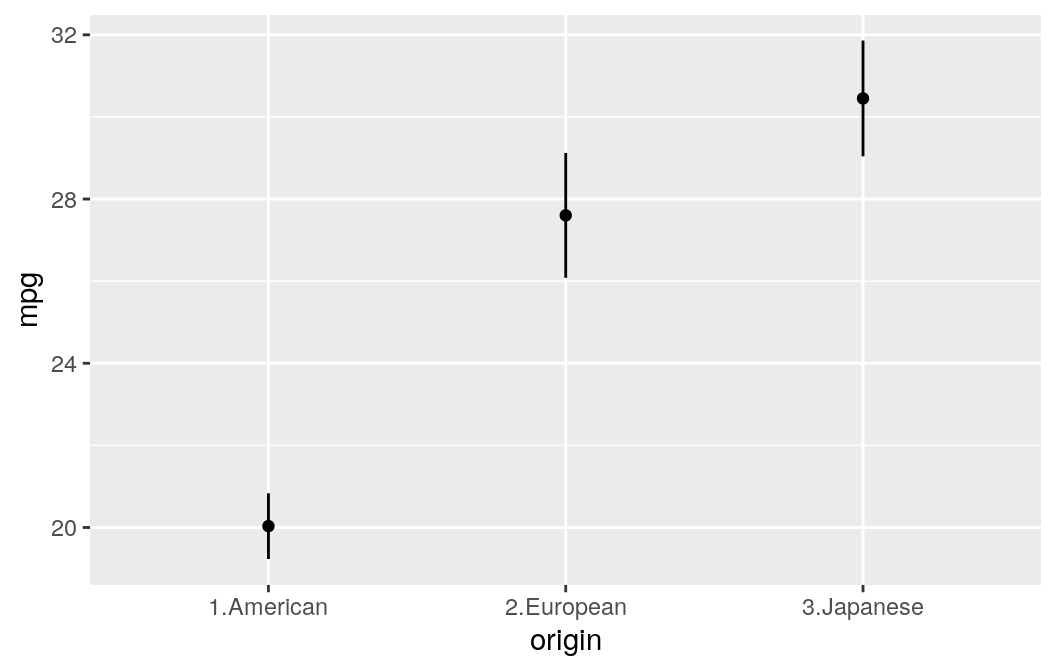
\includegraphics[width=0.6\linewidth]{11Nnet_files/figure-beamer/unnamed-chunk-3-1} \end{center}

\end{frame}

\begin{frame}

\begin{block}{Parameter estimation in the statistical model}

(Maximum likelihood) \vspace{2mm}

\begin{itemize}
\tightlist
\item
  Given \(n\) independent pairs of covariates and responses
  \(\{x_i, y_i\}\), the log-likelihood function of a logistic regression
  model can be written as: \vspace{-2mm}
\end{itemize}

\[ \ln(L(\boldsymbol{\beta}))=l(\boldsymbol{\beta}) =\sum_{i=1}^n \Big ( y_i \ln p_i + (1-y_i) \ln(1 - p_i )\Big ) \ .\]

\begin{itemize}
\tightlist
\item
  Maximiation: set the \(r+1\) partial derivatives (to form the
  gradient) to 0.
\end{itemize}

\small

\begin{itemize}
\tightlist
\item
  No closed form solution, thus we use a
  \emph{\textcolor{red}{gradient-based method}} (the Newton-Raphson or
  \href{https://en.wikipedia.org/wiki/Scoring_algorithm}{Fisher scoring
  algorithm} to find \(\hat\beta\) and \(SD(\hat\beta)\): \[
  \beta^{(t+1)}=\beta^{(t)} + {\boldsymbol F}({\boldsymbol \beta}^{(t)})^{-1} s(\beta^{(t)}) \ ,
  \] where the gradient of the log-likelihood
  \({\boldsymbol s}({\boldsymbol \beta})=\frac{\partial l}{\partial \boldsymbol \beta}\)
  is called the score vector, and here the new quantity
  \({\boldsymbol F}({\boldsymbol \beta}^{(t)})^{-1}\) is called the
  inverse \emph{expected Fisher information matrix}.
\end{itemize}

\end{block}

\end{frame}

\begin{frame}

\begin{block}{The neural network model: architecture and activation
function}

\(~\)

\begin{itemize}
\tightlist
\item
  Remember: in the neural network (NN) version of \emph{linear
  regression}, we had:
  \[ y_1({\boldsymbol x}_i)=w_0+w_1 x_{i1}+\cdots + w_r x_{ir} \ , \]
  with activation function \(\phi_o(x)=x\).
\end{itemize}

\(~\)

\begin{itemize}
\tightlist
\item
  In the NN version of \emph{logistic regression} we instead have the
  \emph{\textcolor{red}{sigmoid activation function}}
  \(\phi_o(x)=\frac{1}{1+\exp(-x)}\), often denoted as \(\sigma(x)\).
  Again, we prefer to use \(\hat{y}_1({\boldsymbol x}_i)\) and get:
\end{itemize}

\[ 
\hat{y}_1({\boldsymbol x}_i)= \sigma({\boldsymbol x}_i) = \frac{1}{1+\exp(-(w_0+w_1 x_{i1}+\cdots + w_r x_{ir}))} \in (0,1) \ . 
\]

\end{block}

\end{frame}

\begin{frame}

\begin{block}{Neural networks: loss function and gradient descent}

\vspace{2mm}

\begin{itemize}
\tightlist
\item
  For NNs we use \emph{\textcolor{red}{binomial cross-entropy loss}}
  \[ J({\boldsymbol w})=-\frac{1}{n}\sum_{i=1}^n (y_i\ln({\hat{y}_1({\boldsymbol x}_i)})+(1-y_i)\ln(1-{\hat{y}_1({\boldsymbol x}_i)}) \ , \]
  which is a scaled version of the negative of the binomial
  loglikelihood!
\end{itemize}

\(~\)

\begin{itemize}
\tightlist
\item
  Optimization is done also with
  \emph{\textcolor{red}{gradient descent}}, but we need the chain rule
  (due to the activation function) to get the partial derivatives for
  the gradient direction.
\end{itemize}

\(~\)

\begin{itemize}
\tightlist
\item
  We need the \emph{\textcolor{red}{backpropagation algorithm}}, using
  the activation and loss functions given here.
\end{itemize}

\end{block}

\end{frame}

\begin{frame}[fragile]

\begin{block}{Parameter estimation vs.~network weights}

\(~\)

\tiny

\begin{Shaded}
\begin{Highlighting}[]
\NormalTok{fitlogist =}\StringTok{ }\KeywordTok{glm}\NormalTok{(diabetes }\OperatorTok{~}\StringTok{ }\NormalTok{npreg }\OperatorTok{+}\StringTok{ }\NormalTok{glu }\OperatorTok{+}\StringTok{ }\NormalTok{bp }\OperatorTok{+}\StringTok{ }\NormalTok{skin }\OperatorTok{+}\StringTok{ }\NormalTok{bmi }\OperatorTok{+}\StringTok{ }\NormalTok{ped }\OperatorTok{+}\StringTok{ }\NormalTok{age, }
    \DataTypeTok{data =}\NormalTok{ train, }\DataTypeTok{family =} \KeywordTok{binomial}\NormalTok{(}\DataTypeTok{link =} \StringTok{"logit"}\NormalTok{))}
\KeywordTok{summary}\NormalTok{(fitlogist)}
\end{Highlighting}
\end{Shaded}

\begin{verbatim}
## 
## Call:
## glm(formula = diabetes ~ npreg + glu + bp + skin + bmi + ped + 
##     age, family = binomial(link = "logit"), data = train)
## 
## Deviance Residuals: 
##     Min       1Q   Median       3Q      Max  
## -1.9830  -0.6773  -0.3681   0.6439   2.3154  
## 
## Coefficients:
##              Estimate Std. Error z value Pr(>|z|)    
## (Intercept) -9.773062   1.770386  -5.520 3.38e-08 ***
## npreg        0.103183   0.064694   1.595  0.11073    
## glu          0.032117   0.006787   4.732 2.22e-06 ***
## bp          -0.004768   0.018541  -0.257  0.79707    
## skin        -0.001917   0.022500  -0.085  0.93211    
## bmi          0.083624   0.042827   1.953  0.05087 .  
## ped          1.820410   0.665514   2.735  0.00623 ** 
## age          0.041184   0.022091   1.864  0.06228 .  
## ---
## Signif. codes:  0 '***' 0.001 '**' 0.01 '*' 0.05 '.' 0.1 ' ' 1
## 
## (Dispersion parameter for binomial family taken to be 1)
## 
##     Null deviance: 256.41  on 199  degrees of freedom
## Residual deviance: 178.39  on 192  degrees of freedom
## AIC: 194.39
## 
## Number of Fisher Scoring iterations: 5
\end{verbatim}

\end{block}

\end{frame}

\begin{frame}[fragile]

\tiny

\begin{Shaded}
\begin{Highlighting}[]
\KeywordTok{set.seed}\NormalTok{(}\DecValTok{787879}\NormalTok{)}
\KeywordTok{library}\NormalTok{(nnet)}
\NormalTok{fitnnet =}\StringTok{ }\KeywordTok{nnet}\NormalTok{(diabetes }\OperatorTok{~}\StringTok{ }\NormalTok{npreg }\OperatorTok{+}\StringTok{ }\NormalTok{glu }\OperatorTok{+}\StringTok{ }\NormalTok{bp }\OperatorTok{+}\StringTok{ }\NormalTok{skin }\OperatorTok{+}\StringTok{ }\NormalTok{bmi }\OperatorTok{+}\StringTok{ }\NormalTok{ped }\OperatorTok{+}\StringTok{ }\NormalTok{age, }
    \DataTypeTok{data =}\NormalTok{ train, }\DataTypeTok{linout =} \OtherTok{FALSE}\NormalTok{, }\DataTypeTok{size =} \DecValTok{0}\NormalTok{, }\DataTypeTok{skip =} \OtherTok{TRUE}\NormalTok{, }\DataTypeTok{maxit =} \DecValTok{1000}\NormalTok{, }
    \DataTypeTok{entropy =} \OtherTok{TRUE}\NormalTok{, }\DataTypeTok{Wts =}\NormalTok{ fitlogist}\OperatorTok{$}\NormalTok{coefficients }\OperatorTok{+}\StringTok{ }\KeywordTok{rnorm}\NormalTok{(}\DecValTok{8}\NormalTok{, }\DecValTok{0}\NormalTok{, }\FloatTok{0.1}\NormalTok{))}
\end{Highlighting}
\end{Shaded}

\begin{verbatim}
## # weights:  8
## initial  value 213.575955 
## iter  10 value 89.511044
## final  value 89.195333 
## converged
\end{verbatim}

\begin{Shaded}
\begin{Highlighting}[]
\CommentTok{# entropy=TRUE because default is least squares}
\KeywordTok{cbind}\NormalTok{(fitnnet}\OperatorTok{$}\NormalTok{wts, fitlogist}\OperatorTok{$}\NormalTok{coefficients)}
\end{Highlighting}
\end{Shaded}

\begin{verbatim}
##                     [,1]         [,2]
## (Intercept) -9.773046277 -9.773061533
## npreg        0.103183171  0.103183427
## glu          0.032116832  0.032116823
## bp          -0.004767678 -0.004767542
## skin        -0.001917105 -0.001916632
## bmi          0.083624151  0.083623912
## ped          1.820397792  1.820410367
## age          0.041183744  0.041183529
\end{verbatim}

\(~\)

\normalsize

By setting \texttt{entropy=TRUE} we minimize the cross-entropy loss.

\end{frame}

\begin{frame}[fragile]

\begin{Shaded}
\begin{Highlighting}[]
\KeywordTok{plotnet}\NormalTok{(fitnnet)}
\end{Highlighting}
\end{Shaded}

\begin{center}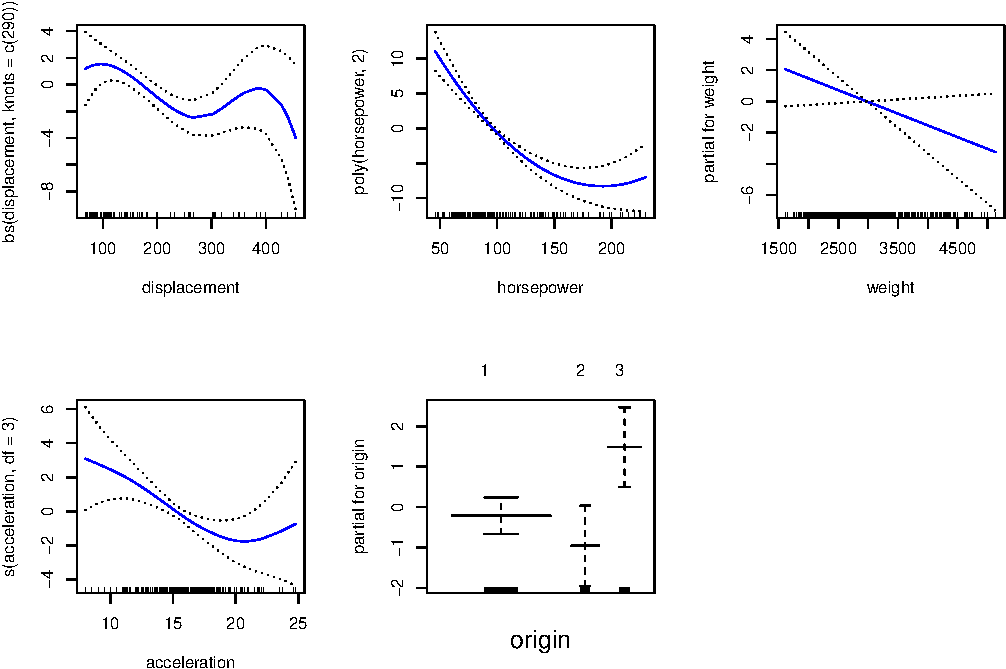
\includegraphics[width=0.9\linewidth]{11Nnet_files/figure-beamer/unnamed-chunk-7-1} \end{center}

\end{frame}

\begin{frame}[fragile]

But, there may also exist local minima.

\(~\)

\scriptsize

\begin{Shaded}
\begin{Highlighting}[]
\KeywordTok{set.seed}\NormalTok{(}\DecValTok{123}\NormalTok{)}
\NormalTok{fitnnet =}\StringTok{ }\KeywordTok{nnet}\NormalTok{(diabetes }\OperatorTok{~}\StringTok{ }\NormalTok{npreg }\OperatorTok{+}\StringTok{ }\NormalTok{glu }\OperatorTok{+}\StringTok{ }\NormalTok{bp }\OperatorTok{+}\StringTok{ }\NormalTok{skin }\OperatorTok{+}\StringTok{ }\NormalTok{bmi }\OperatorTok{+}\StringTok{ }\NormalTok{ped }\OperatorTok{+}\StringTok{ }\NormalTok{age, }
    \DataTypeTok{data =}\NormalTok{ train, }\DataTypeTok{linout =} \OtherTok{FALSE}\NormalTok{, }\DataTypeTok{size =} \DecValTok{0}\NormalTok{, }\DataTypeTok{skip =} \OtherTok{TRUE}\NormalTok{, }\DataTypeTok{maxit =} \DecValTok{10000}\NormalTok{, }
    \DataTypeTok{entropy =} \OtherTok{TRUE}\NormalTok{, }\DataTypeTok{Wts =}\NormalTok{ fitlogist}\OperatorTok{$}\NormalTok{coefficients }\OperatorTok{+}\StringTok{ }\KeywordTok{rnorm}\NormalTok{(}\DecValTok{8}\NormalTok{, }\DecValTok{0}\NormalTok{, }\DecValTok{1}\NormalTok{))}
\end{Highlighting}
\end{Shaded}

\begin{verbatim}
## # weights:  8
## initial  value 24315.298582 
## final  value 12526.062906 
## converged
\end{verbatim}

\begin{Shaded}
\begin{Highlighting}[]
\KeywordTok{cbind}\NormalTok{(fitnnet}\OperatorTok{$}\NormalTok{wts, fitlogist}\OperatorTok{$}\NormalTok{coefficients)}
\end{Highlighting}
\end{Shaded}

\begin{verbatim}
##                     [,1]         [,2]
## (Intercept)   -36.733537 -9.773061533
## npreg         -77.126994  0.103183427
## glu         -2984.409175  0.032116823
## bp          -1835.934259 -0.004767542
## skin         -718.072629 -0.001916632
## bmi          -818.561311  0.083623912
## ped            -8.687473  1.820410367
## age          -773.023878  0.041183529
\end{verbatim}

\end{frame}

\begin{frame}

Why can NN and logistic regression lead to such different results?

\end{frame}

\begin{frame}[fragile]

\begin{block}{Example 3: Categorical outcome (multiclass regression)}

\textbf{Which type of iris species?}

\(~\)

The \texttt{iris} flower data set was introduced by the British
statistician and biologist Ronald Fisher in 1936.

\(~\)

\begin{itemize}
\tightlist
\item
  \textbf{Three plant species}: \{setosa, virginica, versicolor\}.
\item
  \textbf{Four features}: \texttt{Sepal.Length}, \texttt{Sepal.Width},
  \texttt{Petal.Length} and \texttt{Petal.Width}.
\end{itemize}

\(~\)

The aim is to predict the species of an iris plant.

\end{block}

\end{frame}

\begin{frame}

\begin{block}{The statistical model}

\(~\)

We only briefly mentioned multiclass regression in module 4.

\vspace{4mm}

\begin{itemize}
\tightlist
\item
  Assume we have independent observation pairs
  \(({\boldsymbol x}_i, Y_i)\), where the covariate vector
  \({\boldsymbol x}_i\) consists of the same measurements for each
  response category.
\end{itemize}

\(~\)

\begin{itemize}
\tightlist
\item
  Each observation can only belong to one response class,
  \(Y_i \in \{1, \ldots ,C\}\).
\end{itemize}

\(~\)

\begin{itemize}
\tightlist
\item
  \emph{\textcolor{red}{Dummy variable coding}} of the response in a
  \(C\)-dimensional vector:
  \({\boldsymbol y}_i=(0,0,\ldots,0,1,0,\ldots,0)\) with a value of
  \(1\) in the \(c^{th}\) element of \({\boldsymbol y}_i\) if the class
  is \(c\).
\end{itemize}

\end{block}

\end{frame}

\begin{frame}

\begin{itemize}
\tightlist
\item
  Probabilities that the response is category \(c\) for subject \(i\)
  \[p_{ic}=P(Y_i=c)  \ ,\] where \(\sum_{c=1}^C p_{ic}=1\). In
  statistics we do not model \(p_{i1}\), because
  \(p_{i1}=1-\sum_{c=2}^{C} p_{ic}\), and \(\beta_1=0\).
\end{itemize}

\(~\)

\begin{itemize}
\tightlist
\item
  Generalization of the logistic regression model:
  \[p_{ic}=P(Y_i=c)= \frac{\exp({\boldsymbol x}_i^T{\boldsymbol \beta}_c)}{1+\sum_{s=2}^{C}\exp({\boldsymbol x}_i^T{\boldsymbol \beta}_s)}\]
\end{itemize}

\(~\)

\begin{itemize}
\tightlist
\item
  Classification to the class with the highest probability,
  \(\underset{c}{\text{argmax}}(p_{ic})\).
\end{itemize}

\end{frame}

\begin{frame}

\begin{block}{Parameter estimation in the statistical model}

\(~\)

\begin{itemize}
\tightlist
\item
  The likelihood of the multinomial regression model can be written as
  \[ \ln(L({\boldsymbol \beta})\propto \sum_{i=1}^n \sum_{c=1}^C y_{ic}\ln(p_{ic}) \ ,\]
  where \(p_{iC}=1-p_{i1}-p_{i2}-\cdots -p_{i,C-1}\), and the regression
  parameters enter via the \(p_{ic}\)s.
\end{itemize}

\(~\)

\begin{itemize}
\tightlist
\item
  Parameter estimation is done in the same way as for the logistic
  regression, with the Fisher scoring algorithm.
\end{itemize}

\(~\)

\begin{itemize}
\tightlist
\item
  However (and this might be confusing), an efficient function in R also
  relies on neural networks for optimization (see below).
\end{itemize}

\end{block}

\end{frame}

\begin{frame}

\begin{block}{Neural network architecture and activation function}

\vspace{4mm}

\begin{itemize}
\tightlist
\item
  Builds an output layer with \(C\) nodes and corresponding 0/1 targets
  (responses) using the dummy variable coding of the responses, called
  \emph{\textcolor{red}{one-hot coding}}.
\end{itemize}

\vspace{2mm}

\begin{itemize}
\tightlist
\item
  The activation function for the ouput layer is called
  \emph{\textcolor{red}{softmax}}. For each class \(c=1,\ldots, C\) it
  is given as \[
  \hat{y}_c({\boldsymbol x}_i) = \frac{\exp({\boldsymbol x}_i^T{\boldsymbol w}_c)}{\sum_{s=1}^{C}\exp({\boldsymbol x}_i^T{\boldsymbol w}_s)} \ ,
  \] where each \({\boldsymbol w}_s\) is a \(r+1\) dimensional vector of
  weights.
\end{itemize}

\vspace{2mm}

\begin{itemize}
\tightlist
\item
  Note: there is some redundancy here, since
  \(\sum_{c=1}^C {\hat y}_{c}({\boldsymbol x}_i)=1\), so we could have
  had \(C-1\) output nodes, but this is not done.
\end{itemize}

\vspace{2mm}

\begin{itemize}
\tightlist
\item
  The focus of neural networks is not to interpret the weights, and
  there is no need to assume full rank of a matrix with output nodes.
\end{itemize}

\vspace{2mm}

\textbf{Q:} How many parameters are we estimating?

\end{block}

\end{frame}

\begin{frame}

\begin{block}{Neural networks: loss function and gradient descent}

\(~\)

\begin{itemize}
\tightlist
\item
  For parameter estimation we looked at maximizing the log-likelihood of
  the statistical model. For neural networks the negative of the
  multinomial loglikelihood is a scaled version of the
  \emph{\textcolor{red}{categorical cross-entropy loss}}
  \[ J({\boldsymbol w})=-\frac{1}{n}\sum_{i=1}^n\frac{1}{C} \sum_{c=1}^C (y_{ic}\ln({\hat{y}_c({\boldsymbol x}_i)}) \ .\]
\end{itemize}

\(~\)

\begin{itemize}
\tightlist
\item
  The optimization is done using gradient descent, with minor changes
  from what was done for the logistic regression due to the added sum
  and the small change in the activation function.
\end{itemize}

\end{block}

\end{frame}

\begin{frame}[fragile]

\begin{block}{Fitting multinomial regression vs a neural network}

\(~\)

First select a training sample

\scriptsize

\(~\)

\begin{Shaded}
\begin{Highlighting}[]
\KeywordTok{library}\NormalTok{(nnet)}
\KeywordTok{set.seed}\NormalTok{(}\DecValTok{123}\NormalTok{)}
\NormalTok{train =}\StringTok{ }\KeywordTok{sample}\NormalTok{(}\DecValTok{1}\OperatorTok{:}\DecValTok{150}\NormalTok{, }\DecValTok{50}\NormalTok{)}
\NormalTok{iris_train =}\StringTok{ }\NormalTok{ird[train, ]}
\NormalTok{iris_test =}\StringTok{ }\NormalTok{ird[}\OperatorTok{-}\NormalTok{train, ]}
\end{Highlighting}
\end{Shaded}

\(~\)

\normalsize

Then fit the \texttt{nnet()} (by default using the softmax activation
function)

\scriptsize

\begin{Shaded}
\begin{Highlighting}[]
\KeywordTok{set.seed}\NormalTok{(}\DecValTok{1234}\NormalTok{)}
\NormalTok{iris.nnet <-}\StringTok{ }\KeywordTok{nnet}\NormalTok{(species }\OperatorTok{~}\StringTok{ }\NormalTok{., }\DataTypeTok{data =}\NormalTok{ ird, }\DataTypeTok{subset =}\NormalTok{ train, }\DataTypeTok{size =} \DecValTok{0}\NormalTok{, }
    \DataTypeTok{skip =} \OtherTok{TRUE}\NormalTok{, }\DataTypeTok{maxit =} \DecValTok{100}\NormalTok{)}
\end{Highlighting}
\end{Shaded}

\begin{verbatim}
## # weights:  15
## initial  value 105.595764 
## iter  10 value 1.050064
## iter  20 value 0.018814
## iter  30 value 0.003937
## iter  40 value 0.002062
## iter  50 value 0.001460
## iter  60 value 0.000150
## iter  70 value 0.000125
## iter  80 value 0.000110
## final  value 0.000096 
## converged
\end{verbatim}

\end{block}

\end{frame}

\begin{frame}[fragile]

\begin{itemize}
\item
  How many weights have been estimated?
\item
  What does the graph look like?
\end{itemize}

\(~\)

\scriptsize

\begin{Shaded}
\begin{Highlighting}[]
\KeywordTok{summary}\NormalTok{(iris.nnet)}
\end{Highlighting}
\end{Shaded}

\begin{verbatim}
## a 4-0-3 network with 15 weights
## options were - skip-layer connections  softmax modelling 
##  b->o1 i1->o1 i2->o1 i3->o1 i4->o1 
##  36.79   9.69   1.26 -14.33 -13.24 
##  b->o2 i1->o2 i2->o2 i3->o2 i4->o2 
##   5.16  10.10  21.33 -25.47 -12.48 
##  b->o3 i1->o3 i2->o3 i3->o3 i4->o3 
## -42.03 -20.25 -23.12  40.80  25.96
\end{verbatim}

\end{frame}

\begin{frame}

\begin{center}\includegraphics[width=0.9\linewidth]{11Nnet_files/figure-beamer/iris_nnet-1} \end{center}

\end{frame}

\begin{frame}[fragile]

Fitting the multinomial regression. This is also done with nnet, but
using a wrapper \texttt{multinom} (this has its own default settings, so
results are not necessarily the same as above).

\scriptsize

\begin{Shaded}
\begin{Highlighting}[]
\KeywordTok{library}\NormalTok{(caret)}
\NormalTok{fit =}\StringTok{ }\KeywordTok{multinom}\NormalTok{(species }\OperatorTok{~}\StringTok{ }\DecValTok{-1} \OperatorTok{+}\StringTok{ }\NormalTok{., }\DataTypeTok{family =}\NormalTok{ multinomial, }\DataTypeTok{data =}\NormalTok{ iris_train)}
\end{Highlighting}
\end{Shaded}

\begin{verbatim}
## # weights:  15 (8 variable)
## initial  value 54.930614 
## iter  10 value 4.353139
## iter  20 value 0.139411
## iter  30 value 0.065218
## iter  40 value 0.056419
## iter  50 value 0.045548
## iter  60 value 0.020867
## iter  70 value 0.016116
## iter  80 value 0.012952
## iter  90 value 0.012787
## iter 100 value 0.009090
## final  value 0.009090 
## stopped after 100 iterations
\end{verbatim}

\begin{Shaded}
\begin{Highlighting}[]
\KeywordTok{coef}\NormalTok{(fit)}
\end{Highlighting}
\end{Shaded}

\begin{verbatim}
##    Sepal.L.  Sepal.W.  Petal.L.  Petal.W.
## s  -5.91976  21.30247 -12.52073 -2.774511
## v -39.93182 -28.07162  53.73326 41.264390
\end{verbatim}

\end{frame}

\begin{frame}[fragile]

Problem: \texttt{multinom()} seems to fit an intercept \emph{plus} an
offset node (B), thus we have to remove the intercept manually (by
saying \texttt{-1} in the above formula).

\begin{center}\includegraphics[width=0.8\linewidth]{11Nnet_files/figure-beamer/iris_fit-1} \end{center}

\end{frame}

\begin{frame}[fragile]

\begin{block}{The performance of multinomial regression vs nnet}

\(~\)

\scriptsize

\begin{Shaded}
\begin{Highlighting}[]
\NormalTok{testclass =}\StringTok{ }\KeywordTok{predict}\NormalTok{(fit, }\DataTypeTok{new =}\NormalTok{ iris_test)}
\KeywordTok{confusionMatrix}\NormalTok{(}\DataTypeTok{data =}\NormalTok{ testclass, }\DataTypeTok{reference =}\NormalTok{ iris_test}\OperatorTok{$}\NormalTok{species)}\OperatorTok{$}\NormalTok{table}
\end{Highlighting}
\end{Shaded}

\begin{verbatim}
##           Reference
## Prediction  c  s  v
##          c 28  0  0
##          s  0 36  0
##          v  4  0 32
\end{verbatim}

\(~\)

\begin{Shaded}
\begin{Highlighting}[]
\KeywordTok{table}\NormalTok{(}\KeywordTok{predict}\NormalTok{(iris.nnet, iris_test, }\DataTypeTok{type =} \StringTok{"class"}\NormalTok{), iris_test}\OperatorTok{$}\NormalTok{species)}
\end{Highlighting}
\end{Shaded}

\begin{verbatim}
##    
##      c  s  v
##   c 29  0  0
##   s  0 36  0
##   v  3  0 32
\end{verbatim}

\end{block}

\end{frame}

\begin{frame}

For more on multinomial regression with R, check
\href{https://www.r-bloggers.com/\%F0\%9F\%93\%8A-multinomial-regression-in-r/}{here}.

\end{frame}

\begin{frame}

\begin{block}{Summing up}

\(~\)

\begin{enumerate}
\tightlist
\item
  \emph{Multiple linear regression}

  \begin{itemize}
  \tightlist
  \item
    NN with one input layer and one node in the output layer,
  \item
    linear activation function,
  \item
    mean squared loss.
  \end{itemize}
\end{enumerate}

\(~\)

\begin{enumerate}
\setcounter{enumi}{1}
\tightlist
\item
  \emph{Logistic regression} (2 classes)

  \begin{itemize}
  \tightlist
  \item
    NN with one input layer and one node in the output layer,
  \item
    sigmoid activation function,
  \item
    and binary cross-entropy loss.
  \end{itemize}
\end{enumerate}

\(~\)

\begin{enumerate}
\setcounter{enumi}{2}
\tightlist
\item
  \emph{Multinomial regression} (\(C>2\) classes)

  \begin{itemize}
  \tightlist
  \item
    NN with one input layer and \(C\) nodes in the output layer,
  \item
    softmax activation function,
  \item
    categorical cross-entropy loss.
  \end{itemize}
\end{enumerate}

\(~\) \textbf{But:}

\begin{itemize}
\item
  These are only linear models (linear boundaries).
\item
  Parameters (weights) found using gradient descent algorithms where the
  learning rate (step length) must be set.
\end{itemize}

\end{block}

\end{frame}

\begin{frame}{Feedforward networks}
\protect\hypertarget{feedforward-networks}{}

\begin{itemize}
\item
  Connections are only forward in the network, but no feedback
  connections that sends the output of the model back into the network.
\item
  Examples: Linear, logistic and multinomial regression with or without
  any \emph{hidden layers} (between the input and output layers).
\item
  We may have no hidden layer, one (to be studied next), or many.
\item
  Adding \emph{hidden layers} with \emph{non-linear activation
  functions} between the input and output layer will make nonlinear
  statistical models.
\item
  The number of hidden layers is called the \emph{depth} of the network,
  and the number of nodes in a layer is called the \emph{width} of the
  layer.
\end{itemize}

\end{frame}

\begin{frame}

\centering

\includegraphics[width=0.8\textwidth,height=\textheight]{drawNNp3h2o3.png}

\end{frame}

\begin{frame}

\begin{block}{The single hidden layer feedforward network}

\(~\)

The nodes are also called \emph{neurons}.

\(~\)

\textbf{Notation}

\(~\)

\begin{enumerate}
\tightlist
\item
  Inputs (input layer nodes), \(j=1,\dots p\):
  \(x_1, x_2, \ldots, x_p\), or as a vector \({\boldsymbol x}\).
\item
  The nodes \(z_m\) in the hidden layer, \(m=1,\ldots, M\); as vector
  \({\boldsymbol z}^\top=(z_1, \ldots, z_M)\), and the hidden layer
  activation function \(\phi_h\). \[
  z_m({\boldsymbol x})=\phi_h(\alpha_{0m}+\sum_{j=1}^p \alpha_{jm}x_{j})
  \] where \(\alpha_{jm}\) is the
  weight\footnote{We stick with greek letters $\alpha$ and $\beta$ for parameters, but call them weights.}
  from input \(j\) to hidden node \(m\), and \(\alpha_{0m}\) is the bias
  term for the \(m\)th hidden node. The hidden nodes can be thought of
  as \emph{latent variables}.
\end{enumerate}

\end{block}

\end{frame}

\begin{frame}

\begin{enumerate}
\setcounter{enumi}{2}
\tightlist
\item
  The node(s) in the output layer, \(c=1,\ldots C\):
  \(y_1, y_2, \ldots, y_C\), or as vector \({\boldsymbol y}\), and
  output layer activation function \(\phi_o\). \[
  \hat{y}_c({\boldsymbol x})=\phi_o(\beta_{0c}+\sum_{m=1}^M \beta_{mc}z_{m}({\boldsymbol x}))
  \] where \(\beta_{mc}\) is from hidden neuron \(m\) to ouput node
  \(c\), and \(\beta_{0c}\) is the bias term for the \(c\)th output
  node.
\end{enumerate}

\(~\)

\begin{enumerate}
\setcounter{enumi}{3}
\tightlist
\item
  Taken together \[
  \hat{y}_c({\boldsymbol x})=\phi_o(\beta_{0c}+\sum_{m=1}^M \beta_{mc}z_{m})=\phi_o(\beta_{0c}+\sum_{m=1}^M \beta_{mc}\phi_h(\alpha_{0m}+\sum_{j=1}^p \alpha_{jm}x_{j}))
  \]
\end{enumerate}

\end{frame}

\begin{frame}

\textbf{Hands on:}

\(~\)

\begin{itemize}
\tightlist
\item
  Identify \(p, M, C\) in the network figure above, and relate that to
  the \(y_{c}({\boldsymbol x})\) equation.
\end{itemize}

\(~\)

\begin{itemize}
\tightlist
\item
  How many parameters need to be estimated for this network?
\end{itemize}

\(~\)

\begin{itemize}
\tightlist
\item
  What determines the values of \(p\) and \(C\)?
\end{itemize}

\(~\)

\begin{itemize}
\tightlist
\item
  How is \(M\) determined?
\end{itemize}

\end{frame}

\begin{frame}

\begin{block}{Special case: linear activation function for the hidden
layer}

\(~\)

If we assume that \(\phi_h(z)=z\) (linear or identity activiation):

\[
\hat{y}_c({\boldsymbol x})=\phi_o(\beta_{0c}+\sum_{m=1}^M \beta_{mc}(\alpha_{0m}+\sum_{j=1}^p \alpha_{jm}x_{j}))
\]

\(~\) \(~\)

\textbf{Q:} Does this look like something you have seen before?

\(~\)

\textbf{A:}

\end{block}

\end{frame}

\begin{frame}

\begin{block}{Universal approximation property}

\(~\)

\begin{itemize}
\tightlist
\item
  Think of the goal of a feedforward network to approximate some
  function \(f\), mapping our input vector \({\boldsymbol x}\) to an
  output value \({\boldsymbol y}\).
\end{itemize}

\(~\)

\begin{itemize}
\tightlist
\item
  What type of mathematical function can a feedforward neural network
  with one hidden layer and linear output activation represent?
\end{itemize}

\(~\) \pause

The
\emph{\textcolor{red}{universal approximation theorem}}\footnote{Goodfellow et al 2016, Section 6.4.1, https://www.deeplearningbook.org}
says that a feedforward network with \vspace{2mm}

\begin{itemize}
\tightlist
\item
  a \emph{linear output layer}
\item
  at least one hidden layer with a ``squashing'' activation function and
  ``enough'' hidden units
\end{itemize}

\vspace{2mm}

can approximate any (Borel measurable) function from one
finite-dimensional space (our input layer) to another (our output layer)
with any desired non-zero amount of error.

\end{block}

\end{frame}

\begin{frame}

In particular, the universal approximation theorem holds for

\begin{itemize}
\tightlist
\item
  The \textbf{sigmoid} \(\phi(a)=1/(1+\exp(-a))\) (logistic) activation
  functions.
\item
  The \textbf{rectified linear unit (ReLU)} \(\phi_h(a)=\max(0,a)\)
  activation functions
\end{itemize}

in the hidden layer.

\center

\includegraphics[width=0.9\linewidth]{11Nnet_files/figure-beamer/unnamed-chunk-16-1}

\end{frame}

\begin{frame}

\begin{itemize}
\tightlist
\item
  The ReLU activiation function has replaced the sigmoid function as
  default in the hidden layer(s) of a feedforward network.
\end{itemize}

\vspace{2mm}

\begin{itemize}
\tightlist
\item
  Even though a large feedforward network with one hidden layer may be
  able to represent a desired function, we may not be able to estimate
  the parameters of the function:

  \begin{itemize}
  \tightlist
  \item
    we may choose too many or too few nodes in the hidden layer.
  \item
    our optimization routine may fail.
  \item
    we may overfit/underfit the training data.
  \end{itemize}
\end{itemize}

\vspace{2mm}

\begin{itemize}
\tightlist
\item
  Alternative: networks with more than one hidden layer, but fewer total
  number of nodes but more layers. A network with \emph{many hidden
  layers} is called a \emph{\textcolor{red}{deep network}}.
\end{itemize}

\end{frame}

\begin{frame}[fragile]

\begin{block}{The \texttt{nnet} and \texttt{keras} R packages}

\(~\)

\begin{itemize}
\item
  We will use both the rather simple \texttt{nnet} R package by Brian
  Ripley and the currently very popular \texttt{keras} package for deep
  learning (the \texttt{keras} package will be presented later).
  \vspace{2mm}
\item
  \texttt{nnet} fits \emph{one hidden layer} with \emph{sigmoid
  activiation function}. The implementation is not gradient descent, but
  instead BFGS using \texttt{optim}. \vspace{2mm}
\end{itemize}

\begin{itemize}
\item
  Type \texttt{?nnet()} into your R-console to see the arguments of
  \texttt{nnet()}. \vspace{2mm}
\item
  If the response in formula is a factor, an appropriate classification
  network is constructed; this has one output and entropy fit if the
  number of levels is two, and a number of outputs equal to the number
  of classes and a softmax output stage for more levels.
\end{itemize}

\end{block}

\end{frame}

\begin{frame}[fragile]{An example}
\protect\hypertarget{an-example}{}

\begin{block}{Boston house prices}

\textbf{Objective}: To predict the median price of owner-occupied homes
in a given Boston suburb in the mid-1970s using 10 input variables.

This data set is both available in the \texttt{MASS} and \texttt{keras}
R package.

\(~\)

\begin{block}{Preparing the data}

\begin{itemize}
\tightlist
\item
  Only 506, split between 404 training samples and 102 test samples
  (this split already done in the \texttt{keras} library)
\item
  Each feature in the input data (for example, the crime rate) has a
  different scale, some values are proportions, which take values
  between 0 and 1; others take values between 1 and 12, others between 0
  and 100, and so on.
\end{itemize}

\end{block}

\end{block}

\end{frame}

\begin{frame}[fragile]

\scriptsize

\begin{Shaded}
\begin{Highlighting}[]
\KeywordTok{library}\NormalTok{(keras)}
\NormalTok{dataset <-}\StringTok{ }\KeywordTok{dataset_boston_housing}\NormalTok{()}
\KeywordTok{c}\NormalTok{(}\KeywordTok{c}\NormalTok{(train_data, train_targets), }\KeywordTok{c}\NormalTok{(test_data, test_targets)) }\OperatorTok\StringTok{ }\NormalTok{dataset}
\KeywordTok{str}\NormalTok{(train_targets)}
\end{Highlighting}
\end{Shaded}

\begin{verbatim}
##  num [1:404(1d)] 15.2 42.3 50 21.1 17.7 18.5 11.3 15.6 15.6 14.4 ...
\end{verbatim}

\begin{Shaded}
\begin{Highlighting}[]
\KeywordTok{head}\NormalTok{(train_data)}
\end{Highlighting}
\end{Shaded}

\begin{verbatim}
##         [,1] [,2]  [,3] [,4]  [,5]  [,6]  [,7]   [,8] [,9] [,10] [,11]
## [1,] 1.23247  0.0  8.14    0 0.538 6.142  91.7 3.9769    4   307  21.0
## [2,] 0.02177 82.5  2.03    0 0.415 7.610  15.7 6.2700    2   348  14.7
## [3,] 4.89822  0.0 18.10    0 0.631 4.970 100.0 1.3325   24   666  20.2
## [4,] 0.03961  0.0  5.19    0 0.515 6.037  34.5 5.9853    5   224  20.2
## [5,] 3.69311  0.0 18.10    0 0.713 6.376  88.4 2.5671   24   666  20.2
## [6,] 0.28392  0.0  7.38    0 0.493 5.708  74.3 4.7211    5   287  19.6
##       [,12] [,13]
## [1,] 396.90 18.72
## [2,] 395.38  3.11
## [3,] 375.52  3.26
## [4,] 396.90  8.01
## [5,] 391.43 14.65
## [6,] 391.13 11.74
\end{verbatim}

\(~\)

\normalsize

The column names are missing (we could get them by using the Boston
dataset loaded from the MASS library, but they are not relevant here).

\end{frame}

\begin{frame}[fragile]

\begin{itemize}
\tightlist
\item
  To make the optimization easier with gradient based methods do
  \emph{\textcolor{red}{feature-wise normalization}}.
\end{itemize}

\(~\)

\scriptsize

\begin{Shaded}
\begin{Highlighting}[]
\NormalTok{org_train =}\StringTok{ }\NormalTok{train_data}
\NormalTok{mean <-}\StringTok{ }\KeywordTok{apply}\NormalTok{(train_data, }\DecValTok{2}\NormalTok{, mean)}
\NormalTok{std <-}\StringTok{ }\KeywordTok{apply}\NormalTok{(train_data, }\DecValTok{2}\NormalTok{, sd)}
\NormalTok{train_data <-}\StringTok{ }\KeywordTok{scale}\NormalTok{(train_data, }\DataTypeTok{center =}\NormalTok{ mean, }\DataTypeTok{scale =}\NormalTok{ std)}
\NormalTok{test_data <-}\StringTok{ }\KeywordTok{scale}\NormalTok{(test_data, }\DataTypeTok{center =}\NormalTok{ mean, }\DataTypeTok{scale =}\NormalTok{ std)}
\end{Highlighting}
\end{Shaded}

\(~\)

\normalsize

\begin{itemize}
\tightlist
\item
  \textbf{Note}: the quantities used for normalizing the test data are
  computed using the training data. You should never use in your
  workflow any quantity computed on the test data, even for something as
  simple as data normalization.
\end{itemize}

\end{frame}

\begin{frame}[fragile]

Just checking out one hidden layer with 5 units to get going.

\scriptsize

\begin{Shaded}
\begin{Highlighting}[]
\KeywordTok{library}\NormalTok{(nnet)}
\NormalTok{fit5 <-}\StringTok{ }\KeywordTok{nnet}\NormalTok{(train_targets }\OperatorTok{~}\StringTok{ }\NormalTok{., }\DataTypeTok{data =}\NormalTok{ train_data, }\DataTypeTok{size =} \DecValTok{5}\NormalTok{, }\DataTypeTok{linout =} \OtherTok{TRUE}\NormalTok{, }
    \DataTypeTok{maxit =} \DecValTok{1000}\NormalTok{)}
\end{Highlighting}
\end{Shaded}

\begin{verbatim}
## # weights:  76
## initial  value 226623.512265 
## iter  10 value 13091.227910
## iter  20 value 7552.270543
## iter  30 value 6973.052157
## iter  40 value 6028.355978
## iter  50 value 5378.466810
## iter  60 value 5178.772252
## iter  70 value 5041.561467
## iter  80 value 4939.293055
## iter  90 value 4847.552123
## iter 100 value 4728.986223
## iter 110 value 4251.914333
## iter 120 value 3946.017314
## iter 130 value 3632.254547
## iter 140 value 3450.244463
## iter 150 value 3322.303263
## iter 160 value 3241.691501
## iter 170 value 3150.472823
## iter 180 value 3107.807649
## iter 190 value 3042.879662
## iter 200 value 3010.915972
## iter 210 value 2942.119646
## iter 220 value 2811.751015
## iter 230 value 2671.932883
## iter 240 value 2569.244747
## iter 250 value 2536.169071
## iter 260 value 2409.402962
## iter 270 value 2357.404065
## iter 280 value 2332.453029
## iter 290 value 2301.928501
## iter 300 value 2275.486910
## iter 310 value 2271.654139
## iter 320 value 2271.341691
## iter 330 value 2270.864907
## iter 340 value 2269.409714
## iter 350 value 2266.898707
## iter 360 value 2265.562591
## iter 370 value 2263.741643
## iter 380 value 2263.341350
## iter 390 value 2263.335141
## iter 400 value 2263.289326
## iter 410 value 2263.107707
## iter 420 value 2262.977137
## iter 430 value 2262.605492
## iter 440 value 2262.152481
## iter 450 value 2261.282844
## iter 460 value 2260.688788
## iter 470 value 2259.044896
## iter 480 value 2256.705839
## iter 490 value 2256.565541
## iter 500 value 2256.387716
## iter 510 value 2256.218543
## iter 520 value 2256.131616
## iter 530 value 2256.005554
## iter 540 value 2255.945243
## iter 550 value 2255.922524
## iter 560 value 2255.912642
## iter 570 value 2255.901700
## iter 580 value 2255.900781
## final  value 2255.898090 
## converged
\end{verbatim}

\begin{Shaded}
\begin{Highlighting}[]
\KeywordTok{summary}\NormalTok{(fit5)}
\end{Highlighting}
\end{Shaded}

\begin{verbatim}
## a 13-5-1 network with 76 weights
## options were - linear output units 
##   b->h1  i1->h1  i2->h1  i3->h1  i4->h1  i5->h1  i6->h1  i7->h1  i8->h1 
##   71.26   20.97   18.74  -20.16  -10.96  -15.63   26.20  254.52 -118.95 
##  i9->h1 i10->h1 i11->h1 i12->h1 i13->h1 
##  -98.91  245.21   40.35  -63.31 -184.66 
##   b->h2  i1->h2  i2->h2  i3->h2  i4->h2  i5->h2  i6->h2  i7->h2  i8->h2 
##  -11.07   -3.92    4.74  -15.11   -0.35   -3.85    2.55   23.85  -24.67 
##  i9->h2 i10->h2 i11->h2 i12->h2 i13->h2 
##  -16.46    3.18    3.34   -2.47  -21.87 
##   b->h3  i1->h3  i2->h3  i3->h3  i4->h3  i5->h3  i6->h3  i7->h3  i8->h3 
##   -8.67   -0.46   -9.66    0.84    0.04   -0.55   -0.05    0.00   -1.41 
##  i9->h3 i10->h3 i11->h3 i12->h3 i13->h3 
##    1.28   -0.15   -0.28    0.13   -1.09 
##   b->h4  i1->h4  i2->h4  i3->h4  i4->h4  i5->h4  i6->h4  i7->h4  i8->h4 
##   -2.81   -1.97    0.05   -0.05   -0.06    0.16    0.84   -0.26   -0.12 
##  i9->h4 i10->h4 i11->h4 i12->h4 i13->h4 
##    0.19   -0.15   -0.17    0.08   -0.06 
##   b->h5  i1->h5  i2->h5  i3->h5  i4->h5  i5->h5  i6->h5  i7->h5  i8->h5 
##    6.67 -209.31 -112.59 -151.07  235.15 -277.72  271.08 -308.09 -106.76 
##  i9->h5 i10->h5 i11->h5 i12->h5 i13->h5 
##   83.51  -83.42  -61.57   14.81   79.96 
##    b->o   h1->o   h2->o   h3->o   h4->o   h5->o 
##   14.01   -4.99    5.29   42.15   41.37    3.05
\end{verbatim}

\begin{Shaded}
\begin{Highlighting}[]
\NormalTok{pred =}\StringTok{ }\KeywordTok{predict}\NormalTok{(fit5, }\DataTypeTok{newdata =}\NormalTok{ test_data, }\DataTypeTok{type =} \StringTok{"raw"}\NormalTok{)}
\KeywordTok{sqrt}\NormalTok{(}\KeywordTok{mean}\NormalTok{((pred[, }\DecValTok{1}\NormalTok{] }\OperatorTok{-}\StringTok{ }\NormalTok{test_targets)}\OperatorTok{^}\DecValTok{2}\NormalTok{))}
\end{Highlighting}
\end{Shaded}

\begin{verbatim}
## [1] 5.274657
\end{verbatim}

\begin{Shaded}
\begin{Highlighting}[]
\KeywordTok{mean}\NormalTok{(}\KeywordTok{abs}\NormalTok{(pred[, }\DecValTok{1}\NormalTok{] }\OperatorTok{-}\StringTok{ }\NormalTok{test_targets))}
\end{Highlighting}
\end{Shaded}

\begin{verbatim}
## [1] 2.955324
\end{verbatim}

\end{frame}

\begin{frame}[fragile]

\begin{block}{How to find best number of hidden nodes?}

\(~\)

\(\rightarrow\) Cross-validation! (Time-consuming, so only results are
shown below.)

\(~\)

\scriptsize

\begin{Shaded}
\begin{Highlighting}[]
\NormalTok{grid =}\StringTok{ }\KeywordTok{c}\NormalTok{(}\DecValTok{5}\NormalTok{, }\DecValTok{10}\NormalTok{, }\DecValTok{15}\NormalTok{, }\DecValTok{20}\NormalTok{, }\DecValTok{25}\NormalTok{, }\DecValTok{30}\NormalTok{, }\DecValTok{50}\NormalTok{)}
\end{Highlighting}
\end{Shaded}

\(~\)

\center

\includegraphics[width=0.6\linewidth]{11Nnet_files/figure-beamer/unnamed-chunk-23-1}

\end{block}

\end{frame}

\begin{frame}[fragile]

The best model here was the model with 50 nodes, the largest model we
tried. Fitting that model on the full training set and testing on the
test set:

\(~\)

\scriptsize

\begin{Shaded}
\begin{Highlighting}[]
\KeywordTok{library}\NormalTok{(nnet)}
\NormalTok{fit50 <-}\StringTok{ }\KeywordTok{nnet}\NormalTok{(train_targets }\OperatorTok{~}\StringTok{ }\NormalTok{., }\DataTypeTok{data =}\NormalTok{ train_data, }\DataTypeTok{size =} \DecValTok{50}\NormalTok{, }\DataTypeTok{linout =} \OtherTok{TRUE}\NormalTok{, }
    \DataTypeTok{maxit =} \DecValTok{5000}\NormalTok{, }\DataTypeTok{trace =}\NormalTok{ F)}
\CommentTok{# head(summary(fit50))}
\NormalTok{pred =}\StringTok{ }\KeywordTok{predict}\NormalTok{(fit50, }\DataTypeTok{newdata =}\NormalTok{ test_data, }\DataTypeTok{type =} \StringTok{"raw"}\NormalTok{)}
\KeywordTok{sqrt}\NormalTok{(}\KeywordTok{mean}\NormalTok{((pred[, }\DecValTok{1}\NormalTok{] }\OperatorTok{-}\StringTok{ }\NormalTok{test_targets)}\OperatorTok{^}\DecValTok{2}\NormalTok{))}
\end{Highlighting}
\end{Shaded}

\begin{verbatim}
## [1] 6.08656
\end{verbatim}

\begin{Shaded}
\begin{Highlighting}[]
\NormalTok{mae =}\StringTok{ }\KeywordTok{mean}\NormalTok{(}\KeywordTok{abs}\NormalTok{(pred[, }\DecValTok{1}\NormalTok{] }\OperatorTok{-}\StringTok{ }\NormalTok{test_targets))}
\NormalTok{mae}
\end{Highlighting}
\end{Shaded}

\begin{verbatim}
## [1] 3.97063
\end{verbatim}

\(~\)

\normalsize

\begin{itemize}
\tightlist
\item
  We could improve this error rate my using deeper networks.
\end{itemize}

\end{frame}

\begin{frame}{Neural network parts}
\protect\hypertarget{neural-network-parts}{}

\(~\)

We now focus on the different elements of neural networks.

\(~\)

\begin{enumerate}
[1)]
\tightlist
\item
  Output layer activation
\item
  Hidden layer activation
\item
  Network architecture
\item
  Loss function
\item
  Optimizers
\end{enumerate}

\end{frame}

\begin{frame}

\begin{block}{1) Output layer activation}

\(~\)

These choices have been guided by solutions in statistics (multiple
linear regression, logistic regression, multiclass regression)

\(~\)

\begin{itemize}
\item
  \emph{\textcolor{red}{Linear activation}}: for \emph{continuous
  outcome} (regression problems) \vspace{2mm}
\item
  \emph{\textcolor{red}{Sigmoid activation}}: for \emph{binary outcome}
  (two-class classification problems) \vspace{2mm}
\item
  \emph{\textcolor{red}{Softmax}}: for \emph{multinomial/categorical
  outcome} (multi-class classification problems)
\end{itemize}

\(~\)

Remark: it is important that the output activation is matched with an
appropriate loss function (see 4).

\end{block}

\end{frame}

\begin{frame}

\begin{block}{2) Hidden layer activation}

\tiny

(See chapter 6.3 in Goodfellow, Bengio, and Courville (2016))

\normalsize

\(~\)

\textbf{Very common}:

\(~\)

\begin{itemize}
\tightlist
\item
  ReLU (\(\phi_h(a)=\max(0,a)\)) is standard choice for deep networks
  (many hidden layers and many nodes) today.
\end{itemize}

\(~\)

\begin{itemize}
\tightlist
\item
  Sigmoid (\(\phi_h(a)=\sigma(a)=1/(1+\exp(-a))\)) or hyperbolic tangent
  (\(\phi_h(a)=\tanh(z)\)).
\end{itemize}

\(~\)

\textbf{Less common}:

\(~\)

\begin{itemize}
\tightlist
\item
  Radial basis functions: as we looked at in Module 9.
\end{itemize}

\(~\)

\begin{itemize}
\tightlist
\item
  Softplus: \(\phi_h(a)=\ln(1+\exp(a))\)
\end{itemize}

\(~\)

\begin{itemize}
\tightlist
\item
  Hard tanh: \(\phi_h(a)=\max(-1,\min(1,a))\)
\end{itemize}

\end{block}

\end{frame}

\begin{frame}

Among all the possibilities, ReLU is nowadays the most popular one. Why?

\(~\)

\begin{itemize}
\item
  The function is piecewise linear, but \emph{in total non-linear}.
\item
  Replacing sigmoid with ReLU is reported to be one of the major changes
  that have improved the performance of the feedforward
  networks\footnote{Goodfellow et al, Section 6.6}.
\item
  Easy to use with gradient descent -- even though the function is not
  differentiable at 0. As we will touch upon later, we don't expect to
  train a network until the gradient is 0. The derivative from the left
  at 0 is 0, and the derivative from the right is
  1\footnote{See Goodfellow et al, Section 6.3 for a discussion on this topic.}.
\end{itemize}

\end{frame}

\begin{frame}

ReLU can also be motivated from biology.

\begin{itemize}
\tightlist
\item
  For some inputs a biological neuron can be completely inactive
\item
  For some inputs a biological neuron output can be proportional to the
  input
\item
  But, most of the time a biological neuron is inactive.
\end{itemize}

According to Goodfellow, Bengio, and Courville (2016) (Section 6.3),
hidden unit design is an \emph{active area of research.}

\centering
\includegraphics[width=0.45\textwidth,height=\textheight]{Action_potential.png}
\small
\url{https://commons.wikimedia.org/wiki/File:Action_potential.svg}

\end{frame}

\begin{frame}

\textbf{Q:} Why can we not just use linear activation function in all
hidden layers?

\textbf{A:} Then each layer would only be able to do linear
transformations of the input data and a deep stack of linear layers
would still implement a linear operation. The activation functions
sigmoid and relu add non-linearity to the model. And, the universial
approximation property is dependent on a squashing type activation
function.

\end{frame}

\begin{frame}

\begin{block}{3) Network architecture}

\(~\)

Network architecture contains three components:

\(~\)

\begin{itemize}
\item
  \emph{\textcolor{red}{Width}}: How many nodes are in each layer of the
  network?
\item
  \emph{\textcolor{red}{Depth}}: How deep is the network (how many
  hidden layers)?
\item
  \emph{\textcolor{red}{Connectivity}}: How are the nodes connected to
  each other?
\end{itemize}

\(~\)

This depends on the problem, and here experience is important.

\(~\)

\begin{itemize}
\tightlist
\item
  We will only consider \emph{feedforward networks}, where all nodes in
  one layer are connected to all the nodes in the next layer. The layers
  are then \emph{fully connected} and \emph{dense}.
\end{itemize}

\end{block}

\end{frame}

\begin{frame}

However, the recent practice, see e.g. Chollet and Allaire (2018),
Section 4.5.6/7 and Goodfellow, Bengio, and Courville (2016), Section 7,
is to

\(~\)

\begin{itemize}
\tightlist
\item
  choose a too large network (too many nodes and/or too many layers) so
  that if trained until convergence (optimum) then the this would result
  in overfitting, and
\end{itemize}

\vspace{2mm}

\begin{itemize}
\tightlist
\item
  then use other means to avoid this (various variants of regularization
  and hyperparameter optimization).
\end{itemize}

\(~\)

This simplifies the choice of network architecture to \emph{choose a
large enough network}.

\end{frame}

\begin{frame}[fragile]

\begin{block}{4) Loss function (``Method'')}

\(~\)

\begin{itemize}
\item
  The choice of the loss function is closely related to the output layer
  activation function.
\item
  To sum up, the popular problem types, output activation and loss
  functions are:
\end{itemize}

\begin{longtable}[]{@{}lll@{}}
\toprule
Problem & Output activation & Loss function\tabularnewline
\midrule
\endhead
Regression & \texttt{linear} & \texttt{mse}\tabularnewline
Classification (C=2) & \texttt{sigmoid} &
\texttt{binary\_crossentropy}\tabularnewline
Classification (C\textgreater{}2) & \texttt{softmax} &
\texttt{categorical\_crossentropy}\tabularnewline
\bottomrule
\end{longtable}

\end{block}

\end{frame}

\begin{frame}

Due to how estimation is done (see below), the loss functions chosen
``need'' to be:

\begin{itemize}
\tightlist
\item
  differentiable
\item
  possible to compute for each single training data point (or a
  mini-batch -- to be explained soon)
\end{itemize}

\(~\)

\end{frame}

\begin{frame}

\begin{block}{5) Optimizors}

\(~\)

Let the unknown parameters be denoted \({\boldsymbol \theta}\) (what we
have previously denotes as \(\alpha\)s and \(\beta\)s), and the loss
function to be minimized \(J({\boldsymbol \theta})\).

\(~\)

\begin{itemize}
\item
  Gradient descent
\item
  Mini-batch stochastic gradient descent (SGD) and true SGD
\item
  Backpropagation
\end{itemize}

\end{block}

\end{frame}

\begin{frame}[fragile]

\begin{block}{Gradient descent}

\(~\)

\textbf{Remember}:

Given the gradient
\(\nabla J({\boldsymbol \theta}^{(t)})\)\footnote{Remember that the gradient is the vector of partial derivatives of the loss function with respect to each of the parameter in the network.}
of the loss function evaluated at the current estimate
\({\boldsymbol \theta}^{(t)}\), then the algorithm estimates the
parameter at the next step as:

\[{\boldsymbol \theta}^{(t+1)}={\boldsymbol \theta}^{(t)} - \lambda \nabla_{\boldsymbol \theta} J({\boldsymbol \theta}^{(t)}) \ , \]

where \(\lambda\) is the \emph{learning rate} (usually a small value).
In \texttt{keras} the default learning rate is \(0.01\).

\vspace{6mm}

\textbf{Q}: Why are we moving in the direction of the negative of the
gradient? Why not the positive?

\textbf{A}:

\end{block}

\end{frame}

\begin{frame}

\begin{block}{Mini-batch stochastic gradient descent (SGD)}

\vspace{2mm}

\begin{itemize}
\item
  In \emph{\textcolor{red}{full gradient descent}}, the loss function is
  computed as a mean over all training examples. \[
  J({\boldsymbol \theta})=\frac{1}{n}\sum_{i=1}^n J({\boldsymbol x}_i, y_i) \ .
  \]
\item
  The gradient is \emph{an average over many individual gradients} from
  the training example. You can think of this as an estimator for an
  expectation.
\end{itemize}

\[
\nabla_{\boldsymbol \theta} J({\boldsymbol \theta})=\frac{1}{n}\sum_{i=1}^n \nabla_{\boldsymbol \theta} J({\boldsymbol x}_i, y_i) \ .
\]

\begin{itemize}
\tightlist
\item
  To build a network that generalizes well, it is important to have many
  training examples, but that would make us spend a lot of time and
  computer resources at calculating each gradient descent step.
\end{itemize}

\end{block}

\end{frame}

\begin{frame}

\emph{\textcolor{red}{Mini-batch stochastic gradient descent}}

\vspace{2mm}

\begin{itemize}
\tightlist
\item
  \textbf{Crucial idea}: The expectation can be approximated by the
  average gradient over just a \emph{mini-batch} (random sample) of the
  observations.
\end{itemize}

\vspace{2mm}

\textbf{Advantages}:

\begin{itemize}
\item
  The optimizer will converge much faster if they can rapidly compute
  approximate estimates of the gradient, instead of slowly computing the
  exact gradient (using all training data).
\item
  Mini-batches may be processed \emph{in parallel}, and the batch size
  is often a power of 2 (32 or 256).
\item
  Small batches also bring in a \emph{regularization effect}, maybe due
  to the variability they bring to the optimization process.
\end{itemize}

\end{frame}

\begin{frame}

In the 3th video (on backpropagation) from 3Blue1Brown there is nice
example of one trajectory from gradient decent and one from SGD (10:10
minutes into the video):
\url{https://www.youtube.com/watch?v=Ilg3gGewQ5U\&list=PLZHQObOWTQDNU6R1_67000Dx_ZCJB-3pi\&index=3}

\end{frame}

\begin{frame}

\textbf{Mini-batch stochastic gradient descent}

\vspace{1mm}

\begin{enumerate}
\tightlist
\item
  Divide all the training samples randomly into \emph{mini-batches}.
\end{enumerate}

\vspace{1mm}

\begin{enumerate}
\setcounter{enumi}{1}
\tightlist
\item
  Until convergence, repeat a) to d)

  \begin{enumerate}
  [a)]
  \tightlist
  \item
    For each mini-batch: Make predictions of the reponses in the
    mini-batch in a \emph{forward pass}.
  \item
    Compute the loss for the training data in this batch.
  \item
    Compute the gradient of the loss with regard to the model's
    parameters (\emph{backward pass}) based on the training data in the
    batch.
    \(\nabla_{\boldsymbol \theta}^* J({\boldsymbol \theta}^{(t)})\)
  \item
    Update all weighs, but just using the average gradient from the
    mini-batch
    \({\boldsymbol \theta}^{(t+1)}={\boldsymbol \theta}^{(t)} - \lambda \nabla_{\boldsymbol \theta} ^* J({\boldsymbol \theta}^{(t)})\)
  \end{enumerate}
\end{enumerate}

\vspace{1mm}

\begin{enumerate}
\setcounter{enumi}{2}
\tightlist
\item
  Network is \emph{trained}; return parameter estimates.
\end{enumerate}

\vspace{6mm}

\textbf{Special case}: \emph{\textcolor{red}{True SGD}} involves only
\emph{\textcolor{red}{one sample}} (mini-batch size 1). \(\rightarrow\)
Mini-batch SGD is a compromise between SGD (one sample per iteration)
and full gradient descent (full dataset per iteration)

\end{frame}

\begin{frame}

\begin{block}{Backpropagation algorithm}

\(~\)

\begin{itemize}
\tightlist
\item
  Computing the analytical expression for the gradient \(\nabla J\) is
  not difficult, but the numerical evaluation may be expensive.
\end{itemize}

\vspace{2mm}

\begin{itemize}
\tightlist
\item
  \emph{\textcolor{red}{Backpropagation}} is a simple and inexpensive
  way to calculate the gradient numerically.
\end{itemize}

\vspace{2mm}

\begin{itemize}
\tightlist
\item
  The \emph{\textcolor{red}{chain rule}} is used to compute derivatives
  of functions of other functions where the derivatives are known, this
  is done efficiently with backpropagation.
\end{itemize}

\vspace{2mm}

\begin{itemize}
\tightlist
\item
  Backpropagation starts with the value of the loss function and works
  backward from the top layers to the bottom layers, applying the chain
  rule to compute the contribution that each parameter has in the loss
  value.
\end{itemize}

\end{block}

\end{frame}

\begin{frame}

More background:

\(~\)

\begin{itemize}
\tightlist
\item
  Mathematical details: Goodfellow, Bengio, and Courville (2016) Section
  6.5.\\
\end{itemize}

\(~\)

\begin{itemize}
\tightlist
\item
  3Blue1Brown videos: \url{https://www.youtube.com/watch?v=Ilg3gGewQ5U}
  and \url{https://www.youtube.com/watch?v=tIeHLnjs5U8}
\end{itemize}

\end{frame}

\begin{frame}

\begin{block}{Variations of SGD --- with adaptive learning rates}

\vspace{2mm}

The learning rate \(\lambda\) is difficult to set. Some ideas for
adaptive learning rates (Goodfellow et al, Chapter 8.5).

\(~\)

\begin{itemize}
\tightlist
\item
  \emph{\textcolor{red}{Momentum term}}: previous gradients are allowed
  to contribute.
\end{itemize}

\(~\)

\begin{itemize}
\tightlist
\item
  \emph{\textcolor{red}{AdaGrad}}: individually adapt the learning rates
  (\(\lambda\)) of all model parameters. The parameters with the largest
  partial derivative of the loss (over all historical squared values)
  have a correspondingly rapid decrease in their learning rate. Nice
  properties when optimization is convex.
\end{itemize}

\(~\)

\begin{itemize}
\tightlist
\item
  \emph{\textcolor{red}{RMSprop}}: modification to AdaGrad in non-convex
  setting. Scales with exponentially weighted moving average instead of
  all historical squared gradient values. This helps to ``forget''
  information from the extreme past.
\end{itemize}

\end{block}

\end{frame}

\begin{frame}

\begin{block}{Regularization}

\(~\)

\begin{itemize}
\tightlist
\item
  Goodfellow, Bengio, and Courville (2016), Chapter 7, define
  regularization as \emph{any modification we make to a learning
  algorithm that is intended to reduce its generalization error but not
  its training error}.
\end{itemize}

\vspace{2mm}

\begin{itemize}
\tightlist
\item
  Remember (module 6): The aim of regularization was to trade
  \emph{increased bias} for \emph{reduced variance}. The ideas was to
  add a penalty to the loss function.
\end{itemize}

\vspace{2mm}

\begin{itemize}
\tightlist
\item
  The penalties we looked at were of type absolute value of parameter
  (\(L_1\), lasso, where we looked at this as model selection) and
  square value of parameter (\(L_2\), ridge regression). This can also
  done for neural networks.
\end{itemize}

\vspace{2mm}

\end{block}

\end{frame}

\begin{frame}

\begin{block}{Regularization in neural networks}

\(~\)

\begin{itemize}
\tightlist
\item
  \emph{Weight decay}: In neural networks this means adding a
  \(L_2\)-penalty to the loss function to \emph{penalize large weights}
  \footnote{see chapter 7.1.1 in Goodfellow et al}:
\end{itemize}

\[ \tilde{J}({\boldsymbol w})= \frac{\alpha}{2}{{\boldsymbol w}^\top{\boldsymbol w}} + J({\boldsymbol w}) \ .\]

\vspace{2mm}

\begin{itemize}
\tightlist
\item
  \emph{Dataset augmentation}: Adding fake data to the dataset, in order
  that the trained model will generalize better. For some learning tasks
  it is straightforward to create fake data. For image data this can be
  done by rotating and scaling the images.
\end{itemize}

\vspace{2mm}

\begin{itemize}
\tightlist
\item
  \emph{Label smoothing}: Motivated by the fact that the training data
  may contain errors in the reponses recorded, and replaced the one-hot
  coding for \(C\) classes with \(\epsilon/(C-1)\) and \(1-\epsilon\)
  for some small \(\epsilon\).
\end{itemize}

\vspace{2mm}

\begin{itemize}
\tightlist
\item
  \emph{Early stopping}
\end{itemize}

\vspace{2mm}

\begin{itemize}
\tightlist
\item
  \emph{Dropout}
\end{itemize}

\end{block}

\end{frame}

\begin{frame}

\begin{block}{Early stopping}

\tiny Based on Goodfellow, Bengio, and Courville (2016), Section 7.8

\normalsize

\(~\)

\begin{itemize}
\tightlist
\item
  The most commonly used for of regularization is \emph{early stopping}.
\end{itemize}

\vspace{2mm}

\begin{itemize}
\tightlist
\item
  If we have chosen a sufficiently large model with the capacity to
  overfit the training data, we would observe that the training error
  decreases steadily during training, but the error on the validation
  set at some point begins to increase.
\end{itemize}

\vspace{2mm}

\begin{itemize}
\tightlist
\item
  If we stop the learning early and return the parameters giving the
  test performance on the validation set, this model would hopefully be
  a better model than if we trained the model until convergence.
\end{itemize}

\vspace{2mm}

\begin{itemize}
\tightlist
\item
  It is possible to think of the number of \emph{training steps} as a
  hyperparameter. This hyperparameter can easily be set, and the cost is
  just the performance on the validation set during training.
  Alternatively, cross-validation can be used.
\end{itemize}

\end{block}

\end{frame}

\begin{frame}

\begin{block}{Dropout}

\tiny

Based on Goodfellow, Bengio, and Courville (2016), Section 7.12, and
Chollet and Allaire (2018) 4.4.3

\normalsize

\(~\)

Dropout was developed by Geoff Hinton and his students.

\(~\)

\begin{itemize}
\item
  During training: randomly \emph{dropout} (set to zero) some outputs in
  a given layer at each iteration. Drop-out rates may be chosen between
  0.2 and 0.5. \vspace{1mm}
\item
  During test: no dropout, but scale done the layer output values by a
  factor equal to the drop-out rate (since now more units are active
  than we had during training). \vspace{1mm}
\item
  Alternatively, the drop-out and scaling (now upscaling) can be done
  during training. \vspace{1mm}
\item
  One way to look at dropout is on the lines of what we did in Module 8
  when we used bootstrapping to produced many data sets and then fitted
  a model to each of them and then took the average (bagging). But
  randomly dropping out outputs in a layer, this can be looked as
  mimicking bagging -- in an efficient way.
\end{itemize}

\end{block}

\end{frame}

\begin{frame}

\begin{block}{Hyperparameter optimization}

\(~\)

\textbf{Hyperparameters}: The network architecture, the number of
batches to run before terminating the optimization, the drop-out rate.

\(~\)

Ways to avoid overfitting:

\vspace{2mm}

\begin{itemize}
\item
  Reduce network size. \vspace{2mm}
\item
  Collect more observations. \vspace{2mm}
\item
  Regularization.
\end{itemize}

\(~\)

It is important that the hyperparameters are chosen on a validation set
or by cross-validation.

\vspace{2mm}

However, a ``popular'' term is \emph{validation-set overfitting} and
refers to using the validation set to decide many hyperparameters, so
many that you may effectively overfit the validation set.

\end{block}

\end{frame}

\begin{frame}{Deep learning}
\protect\hypertarget{deep-learning-1}{}

\emph{Deep Learning is an algorithm which has no theoretical limitations
of what it can learn; the more data you give and the more computational
time you provide, the better it is.}

Geoffrey Hinton (Google)

\end{frame}

\begin{frame}

\begin{block}{Timeline}

(based on Chollet and Allaire (2018))

\(~\)

\begin{itemize}
\tightlist
\item
  Neural networks were investigated in ``toy form'' in the 1950s.
\end{itemize}

\vspace{2mm}

\begin{itemize}
\tightlist
\item
  The first big step was taken in the 1980s when the backpropagation
  algorithm were developed (rediscovered) to perform gradient descent in
  an efficient way.
\end{itemize}

\vspace{2mm}

\begin{itemize}
\tightlist
\item
  In 1989 (Bell Labs, Yann LeCun) used convolutional neural networks to
  classifying handwritten digits, and \emph{LeNet} was used in the US
  Postal Service for reading ZIP codes in the 1990s.
\end{itemize}

\vspace{2mm}

\begin{itemize}
\tightlist
\item
  Not so much activity in the neural network field in the 2000s.
\end{itemize}

\end{block}

\end{frame}

\begin{frame}

\begin{itemize}
\tightlist
\item
  In 2011 neural networks with many layers (and trained with GPUs) were
  performing well on image classification tasks.
\end{itemize}

\vspace{2mm}

\begin{itemize}
\tightlist
\item
  The \href{http://www.image-net.org/}{\emph{ImageNet}} classification
  challenge (classify high resolution colour images into 1k different
  categories after training on 1.4M images) was won by solutions with
  deep convolutional neural networks (convnets). In 2011 the accuracy
  was 74.3\%, in 2012 83.6\% and in 2015 96.4\%.
\end{itemize}

\vspace{2mm}

\begin{itemize}
\tightlist
\item
  From 2012, convnets is the general solution for computer vision tasks.
  Other application areas are natural language processing.
\end{itemize}

\end{frame}

\begin{frame}

\begin{block}{Deep?}

\(~\)

\begin{itemize}
\tightlist
\item
  Deep learning does not mean a deeper understanding, but refers to
  sucessive layers of representations - where the number of layers gives
  the \emph{depth} of the model. Often tens to hundreds of layers are
  used.
\end{itemize}

\vspace{2mm}

\begin{itemize}
\tightlist
\item
  Deep neural networks are not seen as models of the brain, and are not
  related to neurobiology.
\end{itemize}

\vspace{2mm}

\begin{itemize}
\tightlist
\item
  A deep network can be seen as many stages of
  \emph{information-destillation}, where each stage performes a simple
  data transformation. These transformations are not curated by the data
  analyst, but is estimated in the network.
\end{itemize}

\vspace{2mm}

\begin{itemize}
\tightlist
\item
  In contrast, in statistics we first select a set of inputs, then look
  at how these inputs should be transformed, before we apply some
  statistical methods. This transformation step can be called
  \emph{feature engineering} and has been automated in deep learning.
\end{itemize}

\end{block}

\end{frame}

\begin{frame}

\begin{itemize}
\tightlist
\item
  The success of deep learning is dependent upon the breakthroughts

  \begin{itemize}
  \tightlist
  \item
    in \emph{\textcolor{red}{hardware}} development, expecially with
    faster CPUs and massively parallell graphical processing units
    (GPUs).
  \item
    \emph{\textcolor{red}{dataset}} and benchmarks (internet/tech data).
  \item
    improvemets of the \emph{\textcolor{red}{algorithms}}.
  \end{itemize}
\end{itemize}

\(~\)

\begin{itemize}
\tightlist
\item
  Achievements of deep learning includes high quality (near-human to
  super human) image classification, speech recognition, handwriting
  transcription, machine translation, digital assistants, autonomous
  driving, advertise targeting, web searches, playing Go and chess.
\end{itemize}

\end{frame}

\begin{frame}

\begin{block}{The R keras package}

\(~\)

\begin{itemize}
\tightlist
\item
  Earlier good programming skills in C++ was essential to work in deep
  learning. In addition also skills on programming for GPUs were needed.
\end{itemize}

\vspace{2mm}

\begin{itemize}
\tightlist
\item
  With the launch of the Keras library now users may only need basic
  skills in Python or R.
\end{itemize}

\vspace{2mm}

\begin{itemize}
\tightlist
\item
  \href{https://keras.io/}{Keras} can be seen as a way to use LEGO
  bricks in deep learning. To quote the web-page:
\end{itemize}

\vspace{4mm}

\emph{Keras is a high-level neural networks API developed with a focus
on enabling fast experimentation. Being able to go from idea to result
with the least possible delay is key to doing good research.}

\end{block}

\end{frame}

\begin{frame}

More information on the R solution: \url{https://keras.rstudio.com/}

Cheat-sheet for R Keras:
\url{https://github.com/rstudio/cheatsheets/raw/master/keras.pdf}

\end{frame}

\begin{frame}[fragile]

\begin{block}{MNIST dataset}

\(~\)

\begin{itemize}
\tightlist
\item
  This is a larger image version of the handwritten digits data set (a
  different version, ZIP-codes is found under Recommended exercises).
\end{itemize}

\(~\)

\begin{itemize}
\tightlist
\item
  This data analysis is based on
  \url{https://www.math.ntnu.no/emner/TMA4268/2018v/11NN/8-neural_networks_mnist.html}
  and the \texttt{R\ keras} cheat sheet.
\end{itemize}

\end{block}

\end{frame}

\begin{frame}

Objective: classify the digit contained in an image (128 \(\times\) 128
greyscale).

\scriptsize

\includegraphics{11Nnet_files/figure-beamer/unnamed-chunk-25-1.pdf}

\end{frame}

\begin{frame}[fragile]

Labels for the training data:

\scriptsize

\begin{verbatim}
## train_labels
##    0    1    2    3    4    5    6    7    8    9 
## 5923 6742 5958 6131 5842 5421 5918 6265 5851 5949
\end{verbatim}

\end{frame}

\begin{frame}[fragile]

\begin{block}{1. Training and test data}

\(~\)

60 000 images for training and 10 000 images for testing.

\(~\)

\scriptsize

\begin{Shaded}
\begin{Highlighting}[]
\CommentTok{# Training data}
\NormalTok{train_images <-}\StringTok{ }\NormalTok{mnist}\OperatorTok{$}\NormalTok{train}\OperatorTok{$}\NormalTok{x}
\NormalTok{train_labels <-}\StringTok{ }\NormalTok{mnist}\OperatorTok{$}\NormalTok{train}\OperatorTok{$}\NormalTok{y}

\CommentTok{# Test data}
\NormalTok{test_images <-}\StringTok{ }\NormalTok{mnist}\OperatorTok{$}\NormalTok{test}\OperatorTok{$}\NormalTok{x}
\NormalTok{test_labels <-}\StringTok{ }\NormalTok{mnist}\OperatorTok{$}\NormalTok{test}\OperatorTok{$}\NormalTok{y}
\NormalTok{org_testlabels <-}\StringTok{ }\NormalTok{test_labels}
\end{Highlighting}
\end{Shaded}

\(~\)

\normalsize

The \texttt{train\_images} is a tensor (generalization of a matrix) with
3 axis, \texttt{(samples,\ height,\ width)}.

\end{block}

\end{frame}

\begin{frame}[fragile]

\begin{block}{2. Defining the model}

\vspace{2mm}

Using \texttt{keras\_model\_sequential()} we build a model with a stack
of layers. \texttt{layer\_dense()} adds densely connected layers on top
of the input layer. Each sample contains \texttt{28*28=784} pixels (=
input nodes) and 10 features (=output nodes). Adding a bias term
(intercept) is default for \texttt{layer\_dense}.

\scriptsize

\begin{Shaded}
\begin{Highlighting}[]
\NormalTok{network <-}\StringTok{ }\KeywordTok{keras_model_sequential}\NormalTok{() }\OperatorTok\StringTok{ }\KeywordTok{layer_dense}\NormalTok{(}\DataTypeTok{units =} \DecValTok{512}\NormalTok{, }\DataTypeTok{activation =} \StringTok{"relu"}\NormalTok{, }
    \DataTypeTok{input_shape =} \KeywordTok{c}\NormalTok{(}\DecValTok{28} \OperatorTok{*}\StringTok{ }\DecValTok{28}\NormalTok{)) }\OperatorTok\StringTok{ }\KeywordTok{layer_dense}\NormalTok{(}\DataTypeTok{units =} \DecValTok{10}\NormalTok{, }\DataTypeTok{activation =} \StringTok{"softmax"}\NormalTok{)}
\KeywordTok{summary}\NormalTok{(network)}
\end{Highlighting}
\end{Shaded}

\begin{verbatim}
## Model: "sequential"
## ___________________________________________________________________________
## Layer (type)                     Output Shape                  Param #     
## ===========================================================================
## dense (Dense)                    (None, 512)                   401920      
## ___________________________________________________________________________
## dense_1 (Dense)                  (None, 10)                    5130        
## ===========================================================================
## Total params: 407,050
## Trainable params: 407,050
## Non-trainable params: 0
## ___________________________________________________________________________
\end{verbatim}

\vspace{2mm}

\normalsize

As activation function we use \texttt{relu} for the hidden layer, and
\texttt{softmax} for the output layer - since we have 10 classes (where
one is correct each time).

\end{block}

\end{frame}

\begin{frame}[fragile]

\begin{block}{3. Configure the learning process}

\(~\)

We choose

\vspace{2mm}

\begin{itemize}
\item
  The loss function we will use, which is cross-entropy.
\item
  The version of the optimizer, which is RMSprop.
\item
  Which measure (metrics) do we want to monitor in our training phase?
  Here we choose accuracy (=percentage correctly classified).
\end{itemize}

\(~\)

\scriptsize

\begin{Shaded}
\begin{Highlighting}[]
\NormalTok{network }\OperatorTok\StringTok{ }\KeywordTok{compile}\NormalTok{(}\DataTypeTok{optimizer =} \StringTok{"rmsprop"}\NormalTok{, }\DataTypeTok{loss =} \StringTok{"categorical_crossentropy"}\NormalTok{, }
    \DataTypeTok{metrics =} \KeywordTok{c}\NormalTok{(}\StringTok{"accuracy"}\NormalTok{))}
\end{Highlighting}
\end{Shaded}

\end{block}

\end{frame}

\begin{frame}[fragile]

\begin{block}{4. Preprocessing to match with model inputs and outputs}

\(~\)

\begin{itemize}
\item
  The training data is scored in an array of dimension (60000, 28, 28)
  of type integer with values in the {[}0, 255{]} interval. \vspace{2mm}
\item
  The data must be reshaped into the shape the network expects
  (\(28\cdot 28\)). In addition the grey scale values are scales to be
  in the {[}0, 1{]} interval. \vspace{2mm}
\item
  Also, the response must be transformed from 0-10 to a vector of 0s and
  1s (dummy variable coding) aka \emph{one-hot-coding}.
\end{itemize}

\(~\)

\scriptsize

\begin{Shaded}
\begin{Highlighting}[]
\NormalTok{train_images <-}\StringTok{ }\KeywordTok{array_reshape}\NormalTok{(train_images, }\KeywordTok{c}\NormalTok{(}\DecValTok{60000}\NormalTok{, }\DecValTok{28} \OperatorTok{*}\StringTok{ }\DecValTok{28}\NormalTok{))}
\NormalTok{train_images <-}\StringTok{ }\NormalTok{train_images}\OperatorTok{/}\DecValTok{255}
\NormalTok{train_labels <-}\StringTok{ }\KeywordTok{to_categorical}\NormalTok{(train_labels)}

\NormalTok{test_images <-}\StringTok{ }\KeywordTok{array_reshape}\NormalTok{(test_images, }\KeywordTok{c}\NormalTok{(}\DecValTok{10000}\NormalTok{, }\DecValTok{28} \OperatorTok{*}\StringTok{ }\DecValTok{28}\NormalTok{))}
\NormalTok{test_images <-}\StringTok{ }\NormalTok{test_images}\OperatorTok{/}\DecValTok{255}
\NormalTok{test_labels <-}\StringTok{ }\KeywordTok{to_categorical}\NormalTok{(test_labels)}
\end{Highlighting}
\end{Shaded}

\end{block}

\end{frame}

\begin{frame}[fragile]

\begin{block}{5. Fit the model}

\(~\)

\scriptsize

\begin{Shaded}
\begin{Highlighting}[]
\NormalTok{fitted<-network }\OperatorTok\StringTok{ }\KeywordTok{fit}\NormalTok{(train_images, train_labels,}
 \DataTypeTok{epochs =} \DecValTok{30}\NormalTok{, }\DataTypeTok{batch_size =} \DecValTok{128}\NormalTok{)}
\KeywordTok{library}\NormalTok{(ggplot2)}
\KeywordTok{plot}\NormalTok{(fitted)}\OperatorTok{+}\KeywordTok{ggtitle}\NormalTok{(}\StringTok{"Fitted model"}\NormalTok{)}
\end{Highlighting}
\end{Shaded}

\normalsize

\texttt{epoch} defines how many times you go through your training set
(using mini-batches). See
\href{https://keras.io/getting-started/faq/\#what-does-sample-batch-epoch-mean}{here}
for some documentation.

\centering

\includegraphics[width=0.4\textwidth,height=\textheight]{mnistex.png}

\end{block}

\end{frame}

\begin{frame}[fragile]

\begin{block}{6. Evaluation and prediction}

\(~\)

\scriptsize

\begin{Shaded}
\begin{Highlighting}[]
\NormalTok{network }\OperatorTok\StringTok{ }\KeywordTok{evaluate}\NormalTok{(test_images, test_labels)}
\NormalTok{testres =}\StringTok{ }\NormalTok{network }\OperatorTok\StringTok{ }\KeywordTok{predict_classes}\NormalTok{(test_images)}
\CommentTok{# $loss [1] 0.1194063 $acc [1] 0.9827}
\KeywordTok{confusionMatrix}\NormalTok{(}\KeywordTok{factor}\NormalTok{(testres), }\KeywordTok{factor}\NormalTok{(org_testlabels))}
\end{Highlighting}
\end{Shaded}

\begin{Shaded}
\begin{Highlighting}[]
\NormalTok{Confusion Matrix and Statistics}

\NormalTok{          Reference}
\NormalTok{Prediction    }\DecValTok{0}    \DecValTok{1}    \DecValTok{2}    \DecValTok{3}    \DecValTok{4}    \DecValTok{5}    \DecValTok{6}    \DecValTok{7}    \DecValTok{8}    \DecValTok{9}
         \DecValTok{0}  \DecValTok{971}    \DecValTok{0}    \DecValTok{3}    \DecValTok{0}    \DecValTok{1}    \DecValTok{2}    \DecValTok{5}    \DecValTok{1}    \DecValTok{1}    \DecValTok{1}
         \DecValTok{1}    \DecValTok{1} \DecValTok{1128}    \DecValTok{2}    \DecValTok{0}    \DecValTok{0}    \DecValTok{0}    \DecValTok{2}    \DecValTok{2}    \DecValTok{2}    \DecValTok{3}
         \DecValTok{2}    \DecValTok{1}    \DecValTok{1} \DecValTok{1009}    \DecValTok{3}    \DecValTok{3}    \DecValTok{0}    \DecValTok{2}    \DecValTok{7}    \DecValTok{2}    \DecValTok{0}
         \DecValTok{3}    \DecValTok{0}    \DecValTok{1}    \DecValTok{2}  \DecValTok{997}    \DecValTok{0}   \DecValTok{11}    \DecValTok{1}    \DecValTok{3}    \DecValTok{4}    \DecValTok{3}
         \DecValTok{4}    \DecValTok{1}    \DecValTok{0}    \DecValTok{2}    \DecValTok{0}  \DecValTok{969}    \DecValTok{1}    \DecValTok{4}    \DecValTok{2}    \DecValTok{3}    \DecValTok{7}
         \DecValTok{5}    \DecValTok{0}    \DecValTok{1}    \DecValTok{0}    \DecValTok{1}    \DecValTok{0}  \DecValTok{871}    \DecValTok{3}    \DecValTok{0}    \DecValTok{1}    \DecValTok{4}
         \DecValTok{6}    \DecValTok{3}    \DecValTok{2}    \DecValTok{2}    \DecValTok{0}    \DecValTok{3}    \DecValTok{4}  \DecValTok{940}    \DecValTok{0}    \DecValTok{1}    \DecValTok{0}
         \DecValTok{7}    \DecValTok{1}    \DecValTok{1}    \DecValTok{4}    \DecValTok{2}    \DecValTok{1}    \DecValTok{0}    \DecValTok{0} \DecValTok{1002}    \DecValTok{2}    \DecValTok{3}
         \DecValTok{8}    \DecValTok{2}    \DecValTok{1}    \DecValTok{7}    \DecValTok{0}    \DecValTok{0}    \DecValTok{2}    \DecValTok{1}    \DecValTok{4}  \DecValTok{953}    \DecValTok{1}
         \DecValTok{9}    \DecValTok{0}    \DecValTok{0}    \DecValTok{1}    \DecValTok{7}    \DecValTok{5}    \DecValTok{1}    \DecValTok{0}    \DecValTok{7}    \DecValTok{5}  \DecValTok{987}

\NormalTok{Overall Statistics}

\NormalTok{               Accuracy }\OperatorTok{:}\StringTok{ }\FloatTok{0.9827}
                 \DecValTok{95}\NormalTok{% CI }\OperatorTok{:}\StringTok{ }\NormalTok{(}\FloatTok{0.9799}\NormalTok{, }\FloatTok{0.9852}\NormalTok{)}
\NormalTok{    No Information Rate }\OperatorTok{:}\StringTok{ }\FloatTok{0.1135}
\NormalTok{    P}\OperatorTok{-}\NormalTok{Value [Acc }\OperatorTok{>}\StringTok{ }\NormalTok{NIR] }\OperatorTok{:}\StringTok{ }\ErrorTok{<}\StringTok{ }\FloatTok{2.2e-16}

\NormalTok{                  Kappa }\OperatorTok{:}\StringTok{ }\FloatTok{0.9808}
\NormalTok{ Mcnemar}\StringTok{'s Test P-Value : NA}
\end{Highlighting}
\end{Shaded}

\end{block}

\end{frame}

\begin{frame}

\begin{block}{Kaggle}

\(~\)

\begin{itemize}
\tightlist
\item
  \href{https://www.kaggle.com/}{Kaggle} has hosted machine-learning
  competitions since 2010, and by looking at solutions to competitions
  it is possible to get an overview of what works.
\end{itemize}

\vspace{2mm}

\begin{itemize}
\tightlist
\item
  In 2016-2017 gradient boosting methods won the competitions with
  structured data (``shallow'' learning problems), while deeplearning
  won perceptual problems (as image classification).
\end{itemize}

\vspace{2mm}

\begin{itemize}
\tightlist
\item
  Kaggle has helped (and is helping) the rise in deep learning.
\end{itemize}

\vspace{2mm}

\begin{itemize}
\tightlist
\item
  Very timely topic: Analysis of COVID-19 data!
\end{itemize}

\end{block}

\end{frame}

\begin{frame}

\begin{block}{Other analyses}

\begin{block}{Boston housing price}

taken from Chollet and Allaire (2018):
\url{https://www.math.ntnu.no/emner/TMA4268/2018v/11NN/11-neural_networks_boston_housing.html}

\end{block}

\begin{block}{Movie data base}

\url{https://www.math.ntnu.no/emner/TMA4268/2018v/11NN/9-neural_networks_imdb.html}

\end{block}

\begin{block}{Reuters data}

\url{https://www.math.ntnu.no/emner/TMA4268/2018v/11NN/10-neural_networks_reuters.html}

\end{block}

\end{block}

\end{frame}

\begin{frame}[fragile]{Summing up}
\protect\hypertarget{summing-up-1}{}

\begin{itemize}
\tightlist
\item
  Feedforward network architecture: mathematical formula - layers of
  multivariate transformed (\texttt{relu}, \texttt{linear},
  \texttt{sigmoid}) inner products - sequentially connected.
\item
  What is the number of parameters that need to be estimated? Intercept
  term (for each layer) is possible and is referred to as ``bias term''.
\item
  Loss function to minimize (on output layer): regression (mean
  squared), classification binary (binary crossentropy), classification
  multiple classes (categorical crossentropy) --- and remember to
  connect to the correct choice of output activiation function: mean
  squared loss goes with linear activiation, binary crossentropy with
  sigmoid, categorical crossentropy with softmax.
\item
  How to minimize the loss function: gradient based (chain rule)
  back-propagation - many variants.
\item
  Technicalities: \texttt{nnet} and \texttt{keras} in R; Piping
  sequential layers, piping to estimation and then to evaluation
  (metrics).
\end{itemize}

\end{frame}

\begin{frame}{References and further reading}
\protect\hypertarget{references-and-further-reading}{}

\begin{itemize}
\tightlist
\item
  \url{https://youtu.be/aircAruvnKk} from 3BLUE1BROWN - 4 videos - using
  the MNIST-data set as the running example
\item
  Look at how the hidden layer behave:
  \url{https://playground.tensorflow.org}
\item
  Friedman, Hastie, and Tibshirani (2001),Chapter 11: Neural Networks
\item
  Efron and Hastie (2016), Chapter 18: Neural Networks and Deep Learning
\item
  Chollet and Allaire (2018)
\item
  Goodfellow, Bengio, and Courville (2016) (to be used in IT3030)
  \url{https://www.deeplearningbook.org/}
\item
  Explaining backpropagation
  \url{http://neuralnetworksanddeeplearning.com/chap2.html}
\item
  Slides from MA8701 (Thiago Martins)
  \url{https://www.math.ntnu.no/emner/MA8701/2019v/DeepLearning/}
\end{itemize}

\end{frame}

\begin{frame}{Acknowledgements}
\protect\hypertarget{acknowledgements-1}{}

\hypertarget{refs}{}
\leavevmode\hypertarget{ref-kerasR}{}%
Chollet, François, and J. J. Allaire. 2018. \emph{Deep Learning with R}.
Manning Press. \url{https://www.manning.com/books/deep-learning-with-r}.

\leavevmode\hypertarget{ref-casi}{}%
Efron, Bradley, and Trevor Hastie. 2016. \emph{Computer Age Statistical
Inference - Algorithms, Evidence, and Data Science}. Cambridge
University Press.

\leavevmode\hypertarget{ref-ESL}{}%
Friedman, Jerome, Trevor Hastie, and Robert Tibshirani. 2001. \emph{The
Elements of Statistical Learning}. Vol. 1. Springer series in statistics
New York.

\leavevmode\hypertarget{ref-goodfellow}{}%
Goodfellow, Ian, Yoshua Bengio, and Aaron Courville. 2016. \emph{Deep
Learning}. MIT Press.

\end{frame}

\end{document}
